\documentclass[twoside,14Q,uplatex,dvipdfmx]{jsarticle}
\pagestyle{myheadings}
%\markboth{###title####}{Contemporary and Applied Philosophy Vol. #}
\setcounter{page}{1}
\title{グラウンドの論理とグラウンド理論的同値性%\thanks{\textit{CAP}  Vol. # (####) pp. #-#. 受理日 ####.##.## 採用日 ####.##.##}
}
\author{坪井祥吾}

\date{}

%パッケージ
\usepackage{amsmath}
\usepackage{amsthm}
\usepackage{amssymb}
\usepackage{graphicx}
\usepackage{url}
\usepackage{mathrsfs}

%証明図
\usepackage{bussproofs} 
\newenvironment{bprooftree}
  {\leavevmode\hbox\bgroup}
  {\DisplayProof\egroup}

%tikz
\usepackage{tikz}
\usetikzlibrary{intersections, calc, arrows.meta}
\allowdisplaybreaks[1]

%定理環境
\theoremstyle{definition}
\newtheorem{dfn}{定義}
\newtheorem{thm}{定理}
\newtheorem{lem}{補題}
\newtheorem{fact}{事実}
\newtheorem{prop}{命題}
\newtheorem*{lem*}{}

%ハイパーリンク
\usepackage{hyperref}

\begin{document}

\maketitle

%\section*{著者情報}
%\noindent ###auhtor### (###position###  ####mail address###)

\begin{abstract}
In recent years, there have been surges of interest in \emph{constitutive} explanation. This kind of explanation is distinct from a \emph{causal} explanation. For example, ``Jack is evil because he killed a lot of people'' is a constitutive explanation. In this case, the explanans does not cause the explanandum, but instead, constitutes the explanandum. Metaphysicians refer to this kind of explanation as ``ground'' and study its logical features and connections with other notions.  The purpose of this paper is to review the recent studies on the logical features of ground. These studies typically aim to construct the logic of ground, and this paper surveys its proof theory. With this, the following questions will be explored. What logical features does ground have? What are logically complex propositions grounded in? What do logically complex propositions ground? 

Examining these three questions, we can distinguish between the pure logic and the impure logic of ground. The former concerns the first question, and the latter concerns the second and third questions. With few exceptions, philosophers agree with the pure logic of ground. However, controversies arise in the impure logic of ground, and many philosophers have proposed different systems. Moreover, these systems differ concerning the rules that determine the logical behavior of ground. It is important because such differences imply significant distinctions in philosophical conceptions of ground. Finally, the notion of ``ground-theoretic equivalence,'' a central theme of this paper, has an important role in contouring the differences.
\\

{\flushleft{{Keywords:} The Logic of Ground, Ground-theoretic Equivalence, Hyperintentionality, Relevance}}
\end{abstract}

\section{はじめに}\label{introduction}
日常的・科学的・哲学的文脈において,私たちはしばしば非因果的な説明を行う.次に挙げるような説明が,その典型的な事例である.
	\begin{itemize}
	\item ジャックは悪人だ.というのも,ジャックは大勢の人を殺したからだ.
	\item この窓ガラスが脆いのは,それがしかじかの仕方で結合した分子から構成されているせいである.
	\item $A$かつ$B$が真であるのは,$A$と$B$が両方真であるからだ.
	\item この紙切れが千円札であるのは,それが国立印刷局で印刷されているおかげである.
	\item モトコは痛みを感じている.なぜなら,関連する脳状態が成り立っているからだ.
	\end{itemize}
こうした事例においては,非説明項を成り立たせているような説明項に言及することで,明らかに何らかの説明が行われている.しかし,これらは因果的な説明ではない.たとえばジャックが人を殺したことは,ジャックが悪人であることを引き起こしているわけではないだろう.それでは,これらはどのような種類の説明なのか? こうした説明は,\emph{構成的}[constitutive]ないし\emph{決定的}[determinative]な説明である.すなわち,説明項が成り立つことが,非説明項が成り立つことを構成,ないし決定しているのである.そして近年,この種の構成的・決定的な説明関係は\emph{グラウンド}関係と呼ばれ,盛んに研究されている.たとえば同じ例を用いれば,「ジャックが大勢の人を殺したことが,ジャックが悪人であることをグラウンドする」と言われる.(グラウンド関係の関係項については論争がある (cf. Correia\cite{Correia2020})が,本論では特に何らかの立場にコミットすることはしない.ただし,説明の都合上,グラウンドの関係項を「命題」と呼ぶことにする.)

本論の主題はこのグラウンドである.グラウンドという現象は,上述の例からも分かるようにありふれたものであり,しかしまた雑多でもある.グラウンドの研究は,こうしたありふれた,しかし雑多な現象に統一的な見通しを与えてくれるという点で重要だと言える.そして本論では,特にその論理的側面に注目する.つまり,次のような問いを扱う.グラウンド関係それ自体が持っている論理的な特徴にはどのようなものがあるのか? 論理的に複雑な命題(e.g., $A\land B, \exists xFx$)はどのような形式を持つ命題とグラウンド関係に立つのか? こうした問いは,グラウンド言明のための証明論と意味論を構築することを通じて答えられることになる.本論で焦点を当てるのは,それらのうち証明論,特に真理関数的に複雑なグラウンド言明にかかわる推論規則である.またその際,\emph{グラウンド理論的同値性}[ground-theoretic equivalence]という概念\footnote{グラウンド理論的同値性は,事実的同値性[factual equivalence](Correia\cite{Correia2010}),命題的同値性[propositional equivalence](Correia\cite{Correia2017},IVO同値性 (McDaniel\cite{McDaniel2015}) とも呼ばれる.また,グラウンド理論的同値性の概念は,Dorr\cite{Dorr2016}によって論じられている「identification」の概念と非常によく似た概念である.実際,Correia and Skiles\cite{CorreiaandSkiles2019}やLovett\cite{Lovett2020}はそれら二つの概念を同一のものとして取り扱っている.}が重要な役割を果たすことが以下では明らかになるだろう.本論は,そのグラウンドの証明論とグラウンド理論的同値性を巡る研究状況をサーベイするものである.現在,グラウンドの論理として様々な体系が提案されており,その全体像をつかむのは骨の折れる作業である.本論は,そうしたグラウンドの論理の研究において何が争点となっており,何が解決すべき問題として残されているのかを把握する一助となるはずである.

本論の構成は以下の通りである.\ref{assumption}節では,グラウンドの論理に関する議論におけるいくつかの前提事項が導入される.\ref{plg}節では,Fine\cite{Fine2012a,Fine2012b}が提出しているグラウンドの「純粋な」論理(文記号とグラウンド・オペレータのみを含む論理)を要約する.この「純粋な」論理は,「非純粋な」論理(真理関数や量化子なども扱える論理)を構築する際のいわばベースとなるものである.(「純粋」/「非純粋」の区別はその節で導入する.)そして\ref{truthfunction}-\ref{gte}節で,そうした「非純粋な」論理を構築しようとする際に,グラウンド理論的同値性についての考察が不可欠であることが確かめられる.特に,導入規則や除去規則,そして他のいくつかの規則を立てる際に,グラウンド理論的同値性の概念は本質的に重要である.最後に\ref{iplg}節で,真理関数のためのグラウンドの「非純粋な」論理として提案されているいくつかの体系をそれぞれ要約し,比較する.
%
%
%
\section{三つの区別と二つの形式的特徴}\label{assumption}
本節では,まず,グラウンドに関する三つの区別を導入する.完全[full]/部分的[partial]の区別,厳密[strict]/弱い[weak]の区別,叙実的[factive]/非叙実的[non-factive]の区別である.これらの区別はいずれも,グラウンド言明の形式化において重要である.続いて,グラウンドが持つとされる二つの形式的特徴を確認する.グラウンドは,非単調性,超内包性という性質を持つということが仮定されるのである.特に超内包性は,グラウンド理論的同値性の概念と密接に関係している点で重要である.以下では表記法として,〈.〉を文からグラウンドの関係項(命題)への関数として用いる.たとえば,〈雨が降っている〉は,文「雨が降っている」によって表される命題を表示する.

\subsection{完全なグラウンド,部分的なグラウンド}
まず,グラウンドに関する三つの区別を導入しよう.一つ目は,完全な[full]グラウンドと部分的な[partial]グラウンドの区別である.完全なグラウンド,部分的なグラウンドは,直観的にはそれぞれ次のようなものである.$A_1, A_2, \ldots$が$C$を\emph{完全に}グラウンドするとは,$A_1, A_2, \ldots$が$C$を説明するのに十分である,すなわち$A_1, A_2, \ldots$にそれ以上何も付け加える必要がないということである.一方で,$A$が$C$を\emph{部分的に}グラウンドするとは,いくつかの命題$A_1, A_2, \ldots$が存在して,$A, A_1, A_2, \ldots$が$C$を完全にグラウンドする,ということである(cf. Fine\cite[p.3]{Fine2012b}).

たとえば,〈エリコがギターを演奏している〉は,〈チャットモンチーが演奏中である〉を部分的にグラウンドするだろう.さらに他のメンバーに関する事実などを適切に付け加えると,完全なグラウンドの言明を構成することができる.

\subsection{厳密なグラウンド,弱いグラウンド}
二つ目の区別は,厳密な[strict]グラウンドと弱い[weak]グラウンドの区別である.直観的には,それぞれ次のようなものである.$A_1, A_2, \ldots$が$C$を\emph{厳密に}グラウンドするとは,$C$が成り立つのは$A_1, A_2, \ldots$のおかげだということである.(本論冒頭で示した構成的説明の例は,いずれもこの厳密なグラウンドの事例である.)自己説明は標準的には妥当な説明だとはみなされないため,どんなものも自身を厳密にグラウンドすることはないとされる.つまり,厳密なグラウンドは非反射的である.対して,$A_1, A_2, \ldots$が$C$を\emph{弱く}グラウンドするというのは,$C$が持つ「説明上の役割[explanatory role]」を$A_1, A_2, \ldots$が包摂しているということである(Fine\cite[p.3]{Fine2012b}).すなわち,$A_1, A_2, \ldots$が$C$を弱くグラウンドするというのは,$C$が説明するものをすべて$A_1, A_2, \ldots$も説明する,ということである\footnote{ただし,deRosset\cite[pp.715--8]{deRosset2014}はこの特徴づけは失敗していると論じている.さらにdeRossetは,弱いグラウンドについて提案されているいかなる特徴づけも失敗しており,それゆえ弱いグラウンドの概念は維持できないと結論づけけている.本論では,しかし,弱いグラウンドの概念の\emph{前理論的な}把握はこの特徴づけによって成功していると仮定して議論を進める.弱いグラウンドの\emph{厳密な}特徴づけは,以下で弱いグラウンドに関する推論規則を立てることを通じて与えられるはずである.}.それゆえ,どんな命題も自身と説明上の役割は同一であるので,任意の命題は自身を弱くグラウンドする.すなわち,弱いグラウンドは反射的である\footnote{Correia\cite[p.510]{Correia2017})がFine\cite{Fine2012b}の議論に基づいて定式化している次の二つの実質同値は,弱いグラウンドという概念の理解の助けになるかもしれない.(1) $A_1, A_2, \ldots$が$C$を厳密に完全にグラウンドする $\Leftrightarrow$ (i) $A_1, A_2, \ldots$は$C$を弱くグラウンドし,かつ (ii) $C$が弱く部分的にグラウンドするような$A_i$が存在しない ($i=1, 2, \ldots$).(2) $A_1, A_2, \ldots$が$C$を弱く完全にグラウンドする $\Leftrightarrow$ すべての$B$について,$C$が$B$を厳密に完全にグラウンドするならば$A_1, A_2, \ldots$も$B$を厳密に完全にグラウンドする.}.

たとえば,〈トモヤスとコウジが握手をした〉は〈トモヤスとコウジが和解した〉を厳密に(かつ部分的に)グラウンドするだろう.そして,〈トモヤスとコウジが握手をした〉は〈コウジとトモヤスが握手をした〉を弱く(かつ完全に)グラウンドするだろう.というのも,おそらく,後者の説明上の役割を前者が包摂しているからである.(この場合は特に,それらの説明上の役割は同一だろう.)

従って,完全/部分的の区別と合わせると,計四種類のグラウンドが区別される.つまり,厳密で完全なグラウンド,厳密で部分的なグラウンド,弱く完全なグラウンド,弱く部分的なグラウンドである.ただし以下では,断りなく「厳密にグラウンドする」「弱くグラウンドする」と言うとき,それぞれ厳密で完全なグラウンドと弱く完全なグラウンドが意図されている.

\subsection{叙実的なグラウンド,非叙実的なグラウンド}\label{factivenonfactive}
三つ目の区別は,叙実的[factive]なグラウンドと非叙実的[non-factive]なグラウンドの区別である(上の四種類のグラウンドと合わせれば,計八種類のグラウンドが区別されることになる).\emph{叙実的な}グラウンドは,現実に真である(つまり,実際に成り立っている)命題を結ぶものである.たとえば,〈この紙切れが国立印刷局で印刷されている〉は〈それは千円札である〉を叙実的にグラウンドするだろう.これに対し,\emph{非叙実的な}グラウンドは,単に可能であるような命題や,不可能であるような命題の間にも成り立つようなものである.つまり,グラウンドを非叙実的に解釈すれば,実際には成り立っていないような命題や,成り立ちえないような命題についても語ることができるのである.たとえば,単に可能なケースとして,〈この動物はペガサスである〉は〈空を飛ぶ馬が存在する〉を非叙実的にグラウンドするだろう.また,不可能なケースとして,〈この丸屋根は四角い〉は〈四角い丸屋根が存在する〉を非叙実的にグラウンドするだろう.

実は,叙実的なグラウンドは,非叙実的なグラウンドによって次のように容易に定義できる (cf. Fine\cite[p.49]{Fine2012a}, also cf. Correia\cite{Correia2014,Correia2017}, Kr\"{a}mer\cite{Kramer2018,Kramer2021}, Lovett\cite{Lovett2020}).
\begin{align*}
&A_1, A_2, \cdots はCを叙実的にグラウンドする\\
&\;\;\Leftrightarrow\;\text{(i)}\;A_1, A_2, \cdots, Cはすべて真であり,かつ\;\text{(ii)}\;A_1, A_2, \cdots はCを非叙実的にグラウンドする.
\end{align*}
一方で,逆向きの定義,つまり非叙実的なグラウンドを叙実的なグラウンドによって定義することは,少なくとも容易にはうまくいかない.たとえば,次のような一見もっともらしい定義を想定しよう.
\begin{align*}
&A_1, A_2, \cdots はCを非叙実的にグラウンドする\\
&\;\;\Leftrightarrow\;\;A_1, A_2, \cdots がCを叙実的にグラウンドすることが可能である.
\end{align*}
しかし,この定義は失敗している (cf. Fine\cite[p.49]{Fine2012a}).というのも,〈この丸屋根は四角い〉は〈四角い丸屋根が存在する〉を非叙実的にグラウンドするが,しかし〈この丸屋根は四角い〉が〈四角い丸屋根が存在する〉を叙実的にグラウンドすることは不可能だからである(いかなる可能世界においても,〈この丸屋根は四角い〉と〈四角い丸屋根が存在する〉が真となることはない).もしかすると他の定義が可能かもしれないが,本論ではこれ以上は論じない.重要なのは,叙実的なグラウンドを非叙実的なグラウンドによって定義することが容易にできるという点である.それゆえ,非叙実的なグラウンドに関する議論は,定義によって叙実的なグラウンドに関する議論へと容易に拡張できる.実際,何人かの論者はおそらくこうした考えから,非叙実的なグラウンドを集中的に取り扱っている (cf. Correia\cite{Correia2017}, Kr\"{a}mer\cite{Kramer2018,Kramer2021}, Lovett\cite{Lovett2020})\footnote{一方でFine\cite{Fine2012a,Fine2012b}はグラウンドは第一義的には叙実的なものだとしている.「グラウンドとは,ある\emph{真理}が他の\emph{真理}のおかげで成り立つという関係である.」(Fine[p.1]\cite{Fine2012b},強調筆者)}.本論でもこの方針に従い,主に非叙実的なグラウンドについて論じることにする.以下では,断りなく「グラウンド」と言うときには非叙実的なグラウンドが意味されている.ただし\ref{iplg}節では非叙実的なグラウンドから叙実的なグラウンドへの拡張についても簡単に触れる.

%\subsection{狭義半順序性}\label{strictpartialorder}
%\ref{introduction}節で述べた通り,グラウンドは説明的概念である.そしてこのことから,グラウンド関係は狭義半順序であるとされる.ただしある関係$R$が狭義半順序であるとは,それが\emph{非反射的}($\forall x[\lnot xRx]$)で\emph{非対称的}($\forall x\forall y[xRy\rightarrow\lnot yRx]$)で\emph{推移的}($\forall x\forall y\forall z[xRy\land yRz\rightarrow xRz]$)だということである.説明関係が狭義半順序性を満たすというのはもっともらしいと思われる.というのも,常識的には,説明の機能は私たちの理解を促進することだからである.すると,あるものが自身を説明することや,循環的な説明は私たちの理解を促進しない(非反射性,非対称性)だろうし,鎖をなす説明は私たちの理解を促進する(推移性)だろう.従って,形而上学的説明において言及されるグラウンド関係もまた狭義半順序だと想定することは理にかなっている.\footnote{グラウンド関係が狭義半順序であることへの反例はいくつか提案されている.そうした反例とそれらへの応答についてはThompson\cite{Thompson2020}参照.}.
\subsection{非単調性}\label{nonmonotonic}
続いて,二つの形式的特徴に移ろう.まず,グラウンドは\emph{非単調的}[non-monotonic]であるとされる.つまり,グラウンドされるものと無関係なものはそれをグラウンドできないということである.比較として,古典的な含意関係は単調的である.すなわち,$A_1 ,A_2 ,...$が$C$を含意するとき,前件に任意の$B_1 ,B_2 ,...$を加えても含意関係は保存される.たとえば,〈すべての人間は死ぬ〉と〈ソクラテスは人間である〉は,〈ソクラテスは死ぬ〉を含意する.このとき,前件に無関係な命題(e.g., 〈ブリジストンは日本のタイヤメーカーである〉)を付け加えても,含意関係は保存される.しかしながら,同様のことはグラウンドでは許されない.すなわち,$A_1 ,A_2 ,...$が$C$をグラウンドするときでも,$A_1 ,A_2 ,...,B_1 ,B_2 ,...$が$C$をグラウンドするとは必ずしも言えない.なぜなら,$B_1 ,B_2 ,...$が$C$を説明するのに貢献しないかもしれないからである.たとえば,〈モトコはしかじかの脳状態にある〉が〈モトコは痛みを感じている〉をグラウンドするとしても,前件に無関係なもの(再び,〈ブリジストンは日本のタイヤメーカーである〉)を付け加えると,グラウンド関係は保存されない.つまり,グラウンドが説明的概念である以上,グラウンドするものとされるものとの間に\emph{関連性}がなければならないのである\footnote{本論では扱えないが,関連性論理(特にK3, LP, FDE)とグラウンドの論理の間の関係についてCorreia\cite[pp.42--3]{Correia2014}が論じている.}.

\subsection{超内包性とグラウンド理論的同値}\label{hyperintensional}
続いて,グラウンドは\emph{超内包的}[hyperintensional]文脈を形成するとも言われる.つまり,グラウンド言明においては,内包が同じ(i.e., 必然的に同値な)文の置き換えが真理値を必ずしも保存しないのである.たとえば,〈$p\rightarrow p$〉と〈57は素数ではない〉は,いずれもすべての可能世界で真であるので,必然的に同値である.また,ある数に1以外の約数が存在することはそれが素数でないことを説明する,というもっともらしい原則を仮定すれば,
	\begin{align*}
	〈3\times 19=57〉は〈57は素数ではない〉をグラウンドする,
	\end{align*}
は真である.しかし,このグラウンド言明において,〈57は素数ではない〉をそれと必然的に同値な〈$p\rightarrow p$〉と置き換えると,
	\begin{align*}
	〈3\times 19=57〉は〈p\rightarrow p〉をグラウンドする,
	\end{align*}
となる.このグラウンド言明はおそらく偽である.というのも,〈$3\times 19=57$〉は〈$p\rightarrow p$〉と無関係であり,従っていかなる説明関係もそれらの間には成り立たないからである.

さて,グラウンドが超内包的であるということは,グラウンドの概念が様相概念よりも\emph{きめが細かい}ということを意味する.つまり,〈$p\rightarrow p$〉と〈57は素数ではない〉は様相的観点からは区別されないが,グラウンドの観点からは区別されるのである.これらを区別したくなる直観的な動機は,それらが明らかに「同じことを言っていない」というものであろう.そして,本論の主題の一つである\emph{グラウンド理論的同値}関係は,グラウンドの文脈における「同じことを言っている」関係として意図されたものである.換言すれば,グラウンドの推論において真理値を変えることなく置き換え可能な二つの命題が,グラウンド理論的に同値な命題である (cf. Kr\"{a}mer\cite{Kramer2018,Kramer2021}).それゆえ,〈$p\rightarrow p$〉と〈57は素数ではない〉はグラウンドの文脈で置き換え不可能であるため,それらはグラウンド理論的に同値ではないということになる.

さらに重要なことに,構文的観点からも同様に〈$p\rightarrow p$〉と〈57は素数ではない〉は区別されるということに注意すると,次のことがわかる.つまり,グラウンドが超内包的であるという想定が有意味なものになるためには,単にそれが内包的概念よりもきめが細かいと言うだけでは十分ではない.その上で,それが構文的な同一性よりもきめが\emph{粗い}と言う必要もあるのである.というのも,もしそれが構文的な同一性と同じだけのきめの細かさを持つとすると,私たちは単に構文的な特徴に注目するだけでよいことになり,グラウンドが無用の概念になってしまうからである\footnote{超内包的概念一般に関して,きめの\emph{粗さ}の制限が重要であることについてはBjerring and Schwarz\cite{BjerringandSchwarz2017}を見よ.}.つまり,グラウンドなる概念が考慮に値するものであるためには,グラウンドが持つ超内包性がどの程度のものであるのかを特定する必要があるのである.そして,何と何がグラウンド理論的に同値で,何と何がそうでないのかを教えてくれるようなグラウンド理論的同値性の基準を特定することは,まさにこの点で重要である.
%
%
%
\section{グラウンドの純粋な論理}\label{plg}
本節では,Fine\cite{Fine2012a,Fine2012b}による論理の概要を示す.そこでは,前節で確認した形式的性質を満たすようにグラウンドの論理が構築される.本節で取り上げる論理をいかにして拡張するかという問題には次節以降で取り組む.

まずは,\emph{純粋な}[pure]論理と\emph{非純粋な}[impure]論理という区別を導入しておこう.純粋な論理とは,グラウンドする・される文の内的構造(i.e., 真理関数,様相オペレーター,量化子,等々の現れ方)と無関係に,グラウンド関係の形式的特徴のみによって何が何を導くかを規定するものである.たとえば「$A$が$B$をグラウンドし,$B$が$C$をグラウンドするなら,$A$は$C$をグラウンドする」という規則は純粋な論理に属する.対して非純粋な論理とは,グラウンドする・される文の内的構造を考慮に入れるようなものである.たとえば「$A$と$B$が真なら,$A, B$は$A\land B$をグラウンドする」という規則は非純粋な論理に属する.非純粋な論理は純粋な論理の拡張であるので,まずは純粋な論理を作る必要がある.そして以下で見るFineによる論理は,この純粋な論理である.

\subsection{言語}
私たちが扱う言語は次の記号を含む.文記号 ($p, q, r,\ldots$),連言記号 ($\land$),選言記号 ($\lor$),否定記号 ($\lnot$),ボトム記号 ($\bot$),カンマ,括弧,そして四種類のグラウンド・オペレーターである(表\ref{operator}参照)\footnote{グラウンドは\emph{文オペレーター}として表現される.そうではない立場としては,グラウンドをメタ言語的な記号(演繹関係を示すターンスタイル$\vdash$と類比的なもの)として定式化する者(Poggiolesi\cite{Poggiolesi2016,Poggiolesi2018})もいるが,本論では取り上げることはできない.様々な定式化の仕方についての包括的なサーベイとしてはPoggiolesi\cite{Poggiolesi2020}参照.}.

\begin{table}[htb]
\centering
\caption{四種類のオペレーター}\label{operator}
  \begin{tabular}{l|cc}
    & 厳密な[strict] & 弱い[weak] \\ \hline
   完全な[full] & $<$ & $\leq$ \\
    部分的な[partial] & $\prec$ & $\preceq$ \\
  \end{tabular}
\end{table}

そして,\emph{基本式}を次のように定義する.
	\begin{itemize}
	\item[--] 文記号は基本式である.
	\end{itemize}
任意の基本式は大文字のローマ字$A, B, C,\ldots$によって表す.また,実質含意 ($A\rightarrow B$) と実質同値 ($A\leftrightarrow B$) はそれぞれ,$(\lnot A\lor B), ((\lnot A\lor B)\land(\lnot B\lor A))$と定義される.

基本式の\emph{リスト}は,カンマ「,」で区切られた基本式の有限列とする.リストは単一の基本式からなることも,空であることもある.またリストは,並べられた基本式の順序や反復には鋭敏でない.従って$A, B, C$と$A, C, B$,$A, A, A$と$A$はそれぞれ同一のリストを表す.任意のリストは大文字のギリシア文字$\Gamma, \Delta, \ldots$で表す.その上で,\emph{式}を次のように定義する\footnote{これらの定義のもとでは,たとえば$A \prec(B\prec C)$のような表現はできない.$B\prec C$は基本式ではないからである.この種のグラウンドはメタ・グラウンドと呼ばれる (cf. Litland\cite{Litland2020}).Litland\cite{Litland2018}はメタ・グラウンドのための論理を構築している.}.
	\begin{itemize}
	\item[--] 基本式は式である.
	\item[--] $\Gamma$がリストで$A$が基本式ならば,$(\Gamma\leq A), (\Gamma<A)$は式である.
	\item[--] $A, B$が基本式ならば,$(A\preceq B), (A\prec B)$は式である.
	\item[--] $x, y$が式ならば,$(x\land y), (x\lor y), \lnot x$は式である.
	\end{itemize}
たとえば,$((A, B, C\leq B)\land(B<A)), ((C\not\prec D)\rightarrow(D\preceq C))$などは式である.ただし,以下では可読性のため,括弧は適当に省略する.また,たとえば$A\not\prec B$は$\lnot(A\prec B)$の省略である.任意の式は小文字のギリシア文字$\phi, \psi, \ldots$によって表す\footnote{以上の定式化はCorreia\cite{Correia2010}やLovett\cite{Lovett2020}のものとほぼ同様である.これはFineによるものとはやや異なるが,その違いは本質的なものではない.}.

以上の言語のもとで,証明体系を定義する.本論ではLovett\cite{Lovett2020}に倣い,標準的な自然演繹の体系としてそれを定式化する.\emph{規則}は,各ノードが式でラベルづけされた,次のような形の木である.

\begin{prooftree}
	\AxiomC{$\phi_1$}
	\AxiomC{$\phi_2$}
	\AxiomC{$\ldots$}
	\TrinaryInfC{$\psi$}
\end{prooftree}

\noindent \emph{証明木}は,こうした規則を順番に適用することで構成される,単一の根を持つ木のことである.省略的に,証明木を次のように書くことがある.

\begin{prooftree}
	\AxiomC{$\phi_1$}
	\AxiomC{$\phi_2$}
	\AxiomC{$\ldots$}
	\TrinaryInfC{$\vdots$}
	\UnaryInfC{$\psi$}
\end{prooftree}

\noindent ただし縦の三点リーダーは,そこで何回かの規則の適用が行われていることを示す.
%
%
%
\subsection{体系}\label{plgrules}
以上の定義を踏まえて,グラウンドの純粋な論理を提示しよう.Fine\cite{Fine2012a,Fine2012b}は四種類のグラウンドをすべてプリミティブなオペレーターとした上で,十二個の規則からなる以下の体系(the Pure Logic of Groundの頭文字をとって\textsc{PLG}と呼ぶ)を提案している.以下で見るように,これらの規則はいずれもグラウンドの持つべき性質をうまく表現している.
\begin{itemize}
\item \textsc{PLG}
\[
\begin{bprooftree}
	\AxiomC{$\Delta <C$}
\LeftLabel{包摂($</\leq$)}
	\UnaryInfC{$\Delta\leq C$}
\end{bprooftree}
\qquad
\begin{bprooftree}
	\AxiomC{$A\prec C$}
\LeftLabel{包摂($\prec/\preceq$)}
	\UnaryInfC{$A\preceq C$}
\end{bprooftree}
\]

\[
\begin{bprooftree}
	\AxiomC{$\Delta, A <C$}
\LeftLabel{包摂($</\prec$)}
	\UnaryInfC{$A\prec C$}
\end{bprooftree}
\qquad
\begin{bprooftree}
	\AxiomC{$\Delta, A\leq C$}
\LeftLabel{包摂($\leq/\preceq$)}
	\UnaryInfC{$A\preceq C$}
\end{bprooftree}
\]

\begin{prooftree}
	\AxiomC{$A_1, A_2, \ldots\leq C$}
	\AxiomC{$A_1\prec C$}
	\AxiomC{$A_2\prec C$}
	\AxiomC{$\ldots$}
\LeftLabel{逆包摂}
	\QuaternaryInfC{$A_1, A_2, \ldots<C$}
\end{prooftree}

\[
\begin{bprooftree}
	\AxiomC{$A\preceq B$}
	\AxiomC{$B\preceq C$}
\LeftLabel{推移性($\preceq/\preceq$)}
	\BinaryInfC{$A\preceq C$}
\end{bprooftree}
\qquad
\begin{bprooftree}
	\AxiomC{$A\preceq B$}
	\AxiomC{$B\prec C$}
\LeftLabel{推移性($\preceq/\prec$)}
	\BinaryInfC{$A\prec C$}
\end{bprooftree}
\]

\begin{prooftree}
	\AxiomC{$A\prec B$}
	\AxiomC{$B\preceq C$}
\LeftLabel{推移性($\prec/\preceq$)}
	\BinaryInfC{$A\prec C$}
\end{prooftree}

\begin{prooftree}
	\AxiomC{$\Delta_1\leq A_1$}
	\AxiomC{$\Delta_2\leq A_2$}
	\AxiomC{$\ldots$}
	\AxiomC{$A_1, A_2, \ldots\leq C$}
\LeftLabel{Cut($\leq$)}
	\QuaternaryInfC{$\Delta_1, \Delta_2, \ldots\leq C$}
\end{prooftree}

\[
\begin{bprooftree}
	\AxiomC{}
\LeftLabel{同一性($\leq$)}
	\UnaryInfC{$A\leq A$}
\end{bprooftree}
\qquad
\begin{bprooftree}
	\AxiomC{$A\prec A$}
\LeftLabel{非反射性($\prec$)}
	\UnaryInfC{$\bot$}
\end{bprooftree}
\]
\end{itemize}

以上の規則に,さらに真理関数に関する古典的な規則を付け加える.古典的な規則に関しては,以下で明示的に利用する次の四つのみを示すに留める.
\begin{itemize}
\item \textsc{Classical Rules}
\[
\begin{bprooftree}
	\AxiomC{$\phi$}
	\AxiomC{$\lnot\phi$}
	\LeftLabel{$\lnot$-E}
	\BinaryInfC{$\bot$}
\end{bprooftree}
\qquad
\begin{bprooftree}
	\AxiomC{$[\lnot\phi]^{u}$}
	\noLine
	\UnaryInfC{$\vdots$}
	\noLine
	\UnaryInfC{$\bot$}
	\LeftLabel{Reductio, $u$}
	\UnaryInfC{$\phi$}
\end{bprooftree}
\]	
\[
\begin{bprooftree}
\AxiomC{$[\phi]^{u}$}
\UnaryInfC{$\vdots$}
\UnaryInfC{$\psi$}
\LeftLabel{$\rightarrow$-I, $u$}
\UnaryInfC{$\phi\rightarrow\psi$}
\end{bprooftree}
\qquad
\begin{bprooftree}
\AxiomC{$\phi\lor\psi$}
	\AxiomC{$[\phi]^{u}$}
	\UnaryInfC{$\vdots$}
	\UnaryInfC{$\rho$}
		\AxiomC{$[\psi]^{v}$}
		\UnaryInfC{$\vdots$}
		\UnaryInfC{$\rho$}
\LeftLabel{$\lor$-E, $u, v$}
\TrinaryInfC{$\rho$}
\end{bprooftree}
\]
\end{itemize}

さらに,以上の規則から次の規則が派生することは重要である.Cut($<$)とAmalgamationはCut($\leq$)と同一性($\leq$)から,推移性($\prec$)は上の三つの推移性から導出される (cf. Fine\cite[pp.6--7]{Fine2012b}).非反射性($<$)は包摂と非反射性($\prec$)から導かれる (cf. Correia\cite[p.511]{Correia2017}).非対称性は包摂と推移性($\prec$)と非反射性($\prec$)から導かれる.

\begin{prooftree}
	\AxiomC{$\Delta_1<A_1$}
	\AxiomC{$\Delta_2<A_2$}
	\AxiomC{$\ldots$}
	\AxiomC{$A_1, A_2, \ldots<C$}
\LeftLabel{Cut($<$)}
	\QuaternaryInfC{$\Delta_1, \Delta_2, \ldots<C$}
\end{prooftree}

\[
\begin{bprooftree}
	\AxiomC{$A\prec B$}
	\AxiomC{$B\prec C$}
\LeftLabel{推移性($\prec/\prec$)}
	\BinaryInfC{$A\prec C$}
\end{bprooftree}
\qquad
\begin{bprooftree}
	\AxiomC{$\Delta, A<A$}
\LeftLabel{非反射性($<$)}
	\UnaryInfC{$\bot$}
\end{bprooftree}
\]

\[
\begin{bprooftree}
	\AxiomC{$A\prec B$}
	\AxiomC{$B\prec A$}
\LeftLabel{非対称性($\prec$)}
	\BinaryInfC{$\bot$}
\end{bprooftree}
\qquad
\begin{bprooftree}
	\AxiomC{$\Delta, A<B$}
	\AxiomC{$\Delta, B<A$}
\LeftLabel{非対称性($<$)}
	\BinaryInfC{$\bot$}
\end{bprooftree}
\]

\begin{prooftree}
	\AxiomC{$\Delta_1\leq C$}
	\AxiomC{$\Delta_2\leq C$}
	\AxiomC{$\ldots$}
\LeftLabel{Amalgamation($\leq$)}
	\TrinaryInfC{$\Delta_1, \Delta_2, \ldots\leq C$}
\end{prooftree}

\begin{prooftree}
	\AxiomC{$\Delta_1<C$}
	\AxiomC{$\Delta_2<C$}
	\AxiomC{$\ldots$}
\LeftLabel{Amalgamation($<$)}
	\TrinaryInfC{$\Delta_1, \Delta_2, \ldots<C$}
\end{prooftree}
%\begin{align}
%&\dfrac{\Delta_1 <A_1 \;\;\; \Delta_2 <A_2 ... \;\;\; A_1,A_2,...<C}{\Delta_1,\Delta_2...<C}   \tag*{Cut($<$)}\\
%&\notag \\
%&\dfrac{A\prec B \;\;\; B\prec C}{A\prec C}   \tag*{推移性($\prec$)}\\
%&\notag \\
%&\dfrac{A\prec B \;\;\; B\prec A}{\bot} \;\;\;\; \dfrac{\Delta ,A<B \;\;\; \Delta ,B<A}{\bot} \tag*{非対称性}\\
%&\notag \\
%&\dfrac{\Delta ,A<A}{\bot}  \tag*{非反射性($<$)}\\
%&\notag \\
%&\dfrac{\Delta_1 \leq C \;\;\; \Delta_2 \leq C ...}{\Delta_1 ,\Delta_2 ,...\leq C} \;\;\;\; \dfrac{\Delta_1 < C \;\;\; \Delta_2 < C ...}{\Delta_1 ,\Delta_2 ,...<C} \tag*{Amalgamation}
%\end{align}

以上の\textsc{PLG}は,グラウンドの概念をうまく捉えている.包摂と逆包摂は,四種類のグラウンドの間の関係をごく自然な仕方で規定している.推移性とCutは,四種類のグラウンドがすべて推移的であると述べている.同一性($\leq$)は弱いグラウンドが反射的な関係であることを,非反射性は厳密なグラウンドが非反射的な関係であることを表現している.非対称性は厳密なグラウンドが非対称的であることを意味する\footnote{
実際,厳密なグラウンドが説明関係であることを思い起こすと,それが推移的で非反射的で非対称的な関係であることが望ましいだろう.というのも,説明が鎖をなすというのは自然な想定であり(推移性),また自己説明や循環的な説明は禁止されるべき(非反射性,非対称性)だからである.また,弱いグラウンドが説明上の役割の包摂関係であることを思い起こすと,それは,包摂関係である以上,推移的で反射的であるはずだろう.
}.最後に,Amalgamationは,命題の集合がいくつかあり,それらがすべて同じ命題$C$を完全にグラウンドするとき,それらの和集合もまた$C$を完全にグラウンドする,という規則である.この規則は,直観的には,「$A$が$C$を説明し,それとは別の仕方で$B$も$C$を説明するとき,$A$と$B$を両方説明項としたような説明もまた成り立つはずだ」という自然な考えを述べたものだと解釈できよう
\footnote{ただし,Amalgamation($<$)のもっともらしさに関しては,たとえばCorreia\cite[pp.38--9]{Correia2014}やdeRosset\cite[p.235]{deRosset2015}が懸念を表明している.しかし本論ではこの点を問題視することはせず,以下でもAmalgamation($<$)を利用する
}.

\textsc{PLG}については以上である.それは直観的な規則によって構成されており,またその妥当性は大半の論者が合意している (cf. Correia\cite{Correia2010,Correia2014,Correia2017}, Kr\"{a}mer\cite{Kramer2018,Kramer2021}, Lovett\cite{Lovett2020}).しかしながら,その有用性が非常に限られていることも明白だろう.というのも,その純粋であるという性質から,グラウンドする・される文の内的構造(どのような真理関数,様相オペレーター,量化オペレーター,等々の現れ方)によって成り立っているようなグラウンドの言明には,\textsc{PLG}は無力だからである.たとえば,$A\land B$や$\exists xFx$のグラウンドが何であるかを,\textsc{PLG}は教えてくれないのである.従って私たちは,\textsc{PLG}を非純粋な論理へと拡張する必要がある.本論では特に,\emph{真理関数}に関する拡張に論点を絞って検討する\footnote{量化子や述語への拡張に関してはFine\cite{Fine2012a}, Correia\cite{Correia2014}, Genco et al.\cite{Gencoetal2021}を参照.様相オペレーターへの拡張の試みは,Rosen\cite{Rosen2010}やLovett\cite{Lovett2020}で示唆されているが,未だ本格的な形ではほとんど行われていない.}.次節では,真理関数への拡張の準備として,導入規則・除去規則の定式化に関していくつかの争点が存在することを確かめる.
%
%
%
\section{真理関数への拡張にむけて(1):導入規則,除去規則}\label{truthfunction}
本節と次節では,\textsc{PLG}を非純粋な論理へ拡張する際のいくつかの論点を概観する.本節で見る通り,真理関数に関する\emph{導入規則,除去規則}を定式化する際,グラウンド理論的同値性についての考察が不可欠なのである (cf. Correia\cite{Correia2017}, Kr\"{a}mer\cite{Kramer2018,Kramer2021}).(次節では,それら以外のいくつかの重要な規則にとっても,グラウンド理論的同値性の概念が重要であることを確かめる.)そうした導入規則・除去規則についての議論を検討することで,グラウンド理論的同値性について真剣に考慮する動機が,さらには,グラウンド理論的同値性についての規則も含んでいるような非純粋な論理を構築するべき動機が得られるだろう.

\subsection{非論争的な部分}
議論に入る前に,いくつかの予備的な定義と規則を導入する.これらはいずれも,どのようなグラウンドの論理の体系を構築するにせよ受け入れるべきであるような,非論争的なものである.まず,真理関数を含む基本式を扱えるようにするため,基本式の定義に次を追加する.
	\begin{itemize}
	\item[--] $x, y$が基本式ならば,$(x\land y), (x\lor y), \lnot x$は基本式である.
	\end{itemize}
さらに,グラウンド理論的同値性を表す式も扱えるように,式の定義に次を追加する.
	\begin{itemize}
	\item[--] $A, B$が基本式ならば,$(A\approx B)$は式である.
	\end{itemize}

加えて,グラウンド理論的同値性を定義する次の規則を認めることにしよう (cf. Lovett\cite{Lovett2020}).

\begin{prooftree}
\AxiomC{}
\LeftLabel{Def($\approx$)}
\UnaryInfC{$A\approx B\leftrightarrow A\leq B\land B\leq A$}
\end{prooftree}

\noindent 弱いグラウンドが説明上の役割の包摂関係として特徴づけられることを思い起こすと,この定義はもっともらしいと言える.というのも,二つの命題$A, B$が説明上の役割を\emph{相互に}包摂するというのは,それらの説明上の役割が同一だということで,これはそれらがグラウンド理論的同値である(i.e., 同じことを言っている)ということに他ならないからである.実際,大半の論者は,(明示的に論じていない場合もあるが,)この規則を妥当だとみなしている (cf. Correia\cite{Correia2010,Correia2016,Correia2017}, Fine\cite{Fine2017b}, Kr\"{a}mer\cite{Kramer2018,Kramer2021}, Lovett\cite{Lovett2020}).

また,グラウンド理論的に同値な式はグラウンドの文脈で真理値を変えることなく置き換え可能である,ということを保証する次の規則,

\begin{prooftree}
\AxiomC{$\Delta<A$}
\AxiomC{$A\approx B$}
\LeftLabel{Substitution-R}
\BinaryInfC{$\Delta<B$}
\end{prooftree}

\begin{prooftree}
\AxiomC{$A_1\approx B_1$}
\AxiomC{$A_2\approx B_2$}
\AxiomC{$\ldots$}
\AxiomC{$A_1, A_2, \ldots<C$}
\LeftLabel{Substitution-L}
\QuaternaryInfC{$B_1, B_2, \ldots<C$}
\end{prooftree}

\noindent も認めることにしよう.グラウンド理論的同値性はグラウンドの文脈で区別されない式同士の同値関係として意図されているため,この規則は妥当とすべきだろう.やはりこの規則も大半の論者が認めるものである (cf. Correia\cite{Correia2010,Correia2016,Correia2017}, Kr\"{a}mer\cite{Kramer2018,Kramer2021}, Lovett\cite{Lovett2020}).

最後に,\emph{弱い}グラウンドの導入規則として,Lovett\cite{Lovett2020}が提案する次のものを想定しよう.
\begin{itemize}
\item \textsc{Introduction Rules($\leq$)}
\[
\begin{bprooftree}
	\AxiomC{}
\LeftLabel{$\lor$-I$_{1}(\leq)$}
	\UnaryInfC{$A\leq A\lor B$}
\end{bprooftree}
\qquad
\begin{bprooftree}
	\AxiomC{}
\LeftLabel{$\lor$-I$_{2}(\leq)$}
	\UnaryInfC{$A\leq A\lor B$}
\end{bprooftree}
\]

\begin{prooftree}
	\AxiomC{}
\LeftLabel{$\land$-I($\leq$)}
	\UnaryInfC{$A, B\leq A\land B$}
\end{prooftree}

\[
\begin{bprooftree}
	\AxiomC{}
\LeftLabel{$\lnot\land$-I$_1(\leq)$}
	\UnaryInfC{$\lnot A\leq\lnot(A\land B)$}
\end{bprooftree}
\qquad
\begin{bprooftree}
	\AxiomC{}
\LeftLabel{$\lnot\land$-I$_2(\leq)$}
	\UnaryInfC{$\lnot B\leq\lnot(A\land B)$}
\end{bprooftree}
\]

\begin{prooftree}
	\AxiomC{}
\LeftLabel{$\lnot\lor$-I($\leq$)}
	\UnaryInfC{$\lnot A, \lnot B\leq\lnot(A\lor B)$}
\end{prooftree}

\begin{prooftree}
	\AxiomC{}
\LeftLabel{$\lnot\lnot$-I($\leq$)}
	\UnaryInfC{$A\leq\lnot\lnot A$}
\end{prooftree}
\end{itemize}
上記の規則は,いくつかの単純な文が,それらからなる真理関数的に複雑な文を弱く完全にグラウンドすることを許す規則である.たとえば$\land$-I($\leq$)は,「連言は連言肢によって弱くグラウンドされる」ということを述べている.このことは,$A\land B$の説明上の役割が$A, B$を合わせたそれに包摂される,という自然な考えを反映している.他の規則も同様である.これらの規則には取り立てて問題はないように思われる.従って,以下ではこれらの導入規則が妥当であるものとして議論を進める\footnote{
この弱いグラウンドの導入規則は,Lovett\cite{Lovett2020}以外によっては明示的に取り上げられていない.しかし,どの論者もこれを妥当だと認めるはずである.本論の以下の議論を先取りすることになるが,そのことは次のようにして分かる.まず\textsc{Introduction Rules($<$)}を認める場合,\textsc{Introduction Rules($\leq$)}は直ちに出てくる.一方で\textsc{Introduction Rules($<$)}を認めない場合,結果するグラウンドの論理に対しては,真理メーカー意味論が適当な意味論である (cf. Fine\cite{Fine2016,Fine2017b}, Correia\cite{Correia2016}).そして真理メーカー意味論において,弱いグラウンドは,グラウンドする文の真理メーカーの集合がグラウンドされる文の真理メーカーの集合に包含されることとして定義される.詳細はここでは論じられないが,この定義のもとで\textsc{Introduction Rules($\leq$)}が妥当になることは容易に確かめられる.
}.

\subsection{厳密なグラウンドに関する導入規則}\label{introductionrules}
さて,以上の定義や規則を利用して,導入規則と除去規則についての議論を見ていこう.以下では,Fine\cite{Fine2012a}が提示する導入規則と除去規則をたたき台として検討していく.はじめに,厳密なグラウンドの導入規則を取り上げよう.Fineが提案するのは,次のようなシンプルな,無前提の導入規則である.これらはもっともらしく見えるかもしれない.
\begin{itemize}
\item \textsc{Introduction Rules$(<)$}
\[
\begin{bprooftree}
	\AxiomC{}
\LeftLabel{$\lor$-I$_{1}(<)$}
	\UnaryInfC{$A<A\lor B$}
\end{bprooftree}
\qquad
\begin{bprooftree}
	\AxiomC{}
\LeftLabel{$\lor$-I$_{2}(<)$}
	\UnaryInfC{$B<A\lor B$}
\end{bprooftree}
\]

\begin{prooftree}
	\AxiomC{}
\LeftLabel{$\land$-I($<$)}
	\UnaryInfC{$A, B<A\land B$}
\end{prooftree}

\[
\begin{bprooftree}
	\AxiomC{}
\LeftLabel{$\lnot\land$-I$_{1}(<)$}
	\UnaryInfC{$\lnot A<\lnot(A\land B)$}
\end{bprooftree}
\qquad
\begin{bprooftree}
	\AxiomC{}
\LeftLabel{$\lnot\land$-I$_{2}(<)$}
	\UnaryInfC{$\lnot B<\lnot(A\land B)$}
\end{bprooftree}
\]

\begin{prooftree}
	\AxiomC{}
\LeftLabel{$\lnot\lor$-I($<$)}
	\UnaryInfC{$\lnot A, \lnot B<\lnot(A\lor B)$}
\end{prooftree}

\begin{prooftree}
	\AxiomC{}
\LeftLabel{$\lnot\lnot$-I($<$)}
	\UnaryInfC{$A<\lnot\lnot A$}
\end{prooftree}
\end{itemize}
上記の規則は,いくつかの単純な文が,それらからなる複合的な文を厳密にグラウンドすることを許す規則である.たとえば$\lor$-I$_{1}$($<$)は,「選言は選言肢の片方によって厳密にグラウンドされる」ということを述べている.このことは,「$A\lor B$が成り立つのは$A$が成り立つおかげである」,という自然な考えを反映している.他の規則も同様に解釈できる.

問題は,このシンプルな導入規則を認めるべきか否かということである.そして,その基準は,次の冪等律と結合律からなるグラウンド理論的同値のリスト(\textsc{Basic Equivalences}と呼ぶことにしよう)を受け入れるかどうかである.
\begin{itemize}
\item \textsc{Basic Equivalences}

\[
\begin{bprooftree}
	\AxiomC{}
	\LeftLabel{A8}
	\UnaryInfC{$A\approx\lnot\lnot A$}
\end{bprooftree}
\qquad
\begin{bprooftree}
	\AxiomC{}
	\LeftLabel{A9}
	\UnaryInfC{$A\approx A\land A$}
\end{bprooftree}
\qquad
\begin{bprooftree}
\AxiomC{}
\LeftLabel{A10}
\UnaryInfC{$A\approx A\lor A$}
\end{bprooftree}
\]
\[
\begin{bprooftree}
	\AxiomC{}
	\LeftLabel{A11}
	\UnaryInfC{$A\land (B\land C)\approx (A\land B)\land C$}
\end{bprooftree}
\qquad
\begin{bprooftree}
	\AxiomC{}
	\LeftLabel{A12}
	\UnaryInfC{$A\lor (B\lor C)\approx (A\lor B)\lor C$}
\end{bprooftree}
\]
\end{itemize}
(正確には,導入規則にかかわるのは冪等律A8, A9, A10のみで,結合律A11とA12は除去規則にかかわる.)

さて,しかしなぜ\textsc{Basic Equivalences}が問題となるのか? たしかに,上記の無前提の導入規則は,\emph{典型的な}適用事例においては直観的であり,\textsc{Basic Equivalences}とは無関係である.たとえば,〈今日は雨である〉は,〈今日は雨である,またはソクラテスは人間である〉を厳密にグラウンドすると言えるだろう.しかしながら,ある\emph{特別な}適用事例においては直観的な判断が難しくなる.すなわち,$A$と$B$がグラウンド理論的に同値であるとき,それらの規則の適用を認めてよいかどうかで判断が分かれるのである.このことを示すKr\"{a}mer\cite[p.788]{Kramer2018}の議論は次の通りである.

\begin{fact}
\textsc{Introduction Rules$(<)$}は\textsc{Basic Equivalences}と不整合である.
\begin{proof}
$\lor$-I$_{1}(<)$とA10が不整合であることのみを示す.他も同様である.$\lor$-I$_{1}(<)$とA10を仮定すると,次のようにして不整合に陥る.
%:$\lor$-I$_{1}(<)$を仮定すると,その特別な適用事例として$A<A\lor A$が導出可能である.ここでさらにA10を仮定すると,Substitution-Rより$A<A$が導出される.しかし,これは厳密なグラウンドの非反射性と不整合である.

\begin{prooftree}
\AxiomC{}
\LeftLabel{$\lor$-I$_1(<)$}
\UnaryInfC{$A<A\lor A$}
	\AxiomC{}
	\LeftLabel{A10}
	\UnaryInfC{$A\lor A\approx A$}
\LeftLabel{Substitution-R}
\BinaryInfC{$A<A$}
\LeftLabel{非反射性($<$)}
\UnaryInfC{$\bot$}
\end{prooftree}

\end{proof}
\end{fact}

要するに,\textsc{Basic Equivalences}を拒否するならば\textsc{Introduction Rules$(<)$}をそのまま認めることができ,逆に\textsc{Basic Equivalences}を認めるならば\textsc{Introduction Rules$(<)$}を受け入れることはできないのである.

%だが,たとえばA10は拒否されるべきだろうか? すなわち,$A$と$A\lor A$はグラウンド理論的に同値でないと言えるだろうか? 重要なのは,この問いに対して肯定的に答えることも,否定的に答えることも,\emph{どちらも}理にかなっているように思われるということである.$A$と$A\lor A$はいわば語り方が違うだけで「同じことを言っている」のだと考えれば,それらはグラウンド理論的に同値だと認めるべきである (cf. Correia\cite{Correia2010,Correia2016}; Fine\cite{Fine2016}).一方で,単なる$A$の現れと,$A$が$\lor$で結ばれて二度現れることの間には本質的な違いがあるのだと考えれば,それらはグラウンド理論的に同値でないとみなすべきだろう (cf. Correia\cite{Correia2017}; Kr\"{a}mer\cite{Kramer2018,Kramer2021}).A9, A11に関しても同様である.

ただし,\textsc{Basic Equivalences}を認めるからといって導入規則を完全に諦める必要はない.その場合は,Lovett\cite{Lovett2020}が提案する通り,導入規則は次のような前提つきのものになる\footnote{Correia\cite{Correia2010}も前提つきの導入規則を提案している.Correiaのものはより強い前提を置いたものであり,たとえば$\lor$の左側導入の前提は$B\not\preceq A$ではなく$A\not\approx A\lor B$である.}.
\begin{itemize}
\item \textsc{Introduction Rules$^{*}(<)$}
\[
\begin{bprooftree}
	\AxiomC{$B\not\preceq A$}
\LeftLabel{$\lor$-I$^{*}_{1}(<)$}
	\UnaryInfC{$A<A\lor B$}
\end{bprooftree}
\qquad
\begin{bprooftree}
	\AxiomC{$A\not\preceq B$}
\LeftLabel{$\lor$-I$^{*}_{2}(<)$}
	\UnaryInfC{$B<A\lor B$}
\end{bprooftree}
\]

\begin{prooftree}
	\AxiomC{$B\not\preceq A$}
	\AxiomC{$A\not\preceq B$}
\LeftLabel{$\land$-I$^{*}$($<$)}
	\BinaryInfC{$A, B<A\land B$}
\end{prooftree}

\[
\begin{bprooftree}
	\AxiomC{$\lnot B\not\preceq\lnot A$}
\LeftLabel{$\lnot\land$-I$^{*}_{1}(<)$}
	\UnaryInfC{$\lnot A<\lnot(A\land B)$}
\end{bprooftree}
\qquad
\begin{bprooftree}
	\AxiomC{$\lnot A\not\preceq\lnot B$}
\LeftLabel{$\lnot\land$-I$^{*}_{2}(<)$}
	\UnaryInfC{$\lnot B<\lnot(A\land B)$}
\end{bprooftree}
\]

\begin{prooftree}
	\AxiomC{$\lnot B\not\preceq\lnot A$}
	\AxiomC{$\lnot A\not\preceq\lnot B$}
\LeftLabel{$\lnot\lor$-I$^{*}$($<$)}
	\BinaryInfC{$\lnot A, \lnot B<\lnot(A\lor B)$}
\end{prooftree}
\end{itemize}
このようにすれば問題のケース,たとえば$\lor$-I$^{*}_{1}(<)$で言えば$A\approx A\lor B$であるケースを適切に排除できる.(二重否定の導入規則は単に除外されていることに注意せよ.)
\begin{proof}
$\lor$-I$^{*}_{1}(<)$を例にとる.$B\not\preceq A$を前提に置くことで$A\not\approx A\lor B$であることが保証できればよい.まずDef($\approx$)より,$A\approx(A\lor B)\leftrightarrow(A\leq(A\lor B))\land((A\lor B)\leq A)$である.しかし$\lor$-I$_{1}(\leq)$より,常に$A\leq A\lor B$である.よって$A\not\approx A\lor B$を保証するには,$A\lor B\not\leq A$であることを言う必要がある.そして次の証明木によって,たしかに$B\not\preceq A$を前提すれば十分であることが分かる.

\begin{prooftree}
\AxiomC{}
\LeftLabel{$\lor$-I$_{1}(\leq)$}
\UnaryInfC{$B\leq A\lor B$}
	\AxiomC{$[A\lor B\leq A]^{u}$}
\LeftLabel{Cut($\leq$)}
\BinaryInfC{$B\leq A$}
\LeftLabel{包摂($\leq/\preceq$)}
\UnaryInfC{$B\preceq A$}
\LeftLabel{$\rightarrow$-I, u}
\UnaryInfC{$A\lor B\leq A\rightarrow B\preceq A$}
\LeftLabel{}
\UnaryInfC{$\vdots$}
\UnaryInfC{$B\not\preceq A\rightarrow A\lor B\not\leq A$}
\end{prooftree}
\end{proof}
%
%
%
\subsection{厳密なグラウンドに関する除去規則}
続いて,除去規則を検討しよう.そのためには,式の定義を次のように拡張する必要がある\footnote{この拡張の仕方はFine\cite{Fine2012a}, Kr\"{a}mer\cite{Kramer2018,Kramer2021}, Lovett\cite{Lovett2020}に従っている.}.
\begin{itemize}
\item[--] $A$が基本式で$\Gamma$が基本式のリストならば,$(A\leq\Gamma)$は式である.
\item[--] $\Delta, \Gamma$が基本式のリストならば,$(\Delta\leq\Gamma)$は式である.
\end{itemize}
ただし,たとえば$\Delta\leq\Gamma$は,各$A_1, A_2, \ldots\in\Gamma$に対して$\Delta_1\cup\Delta_2\cup\cdots=\Delta$なる$\Delta_1, \Delta_2, \cdots$が存在して,$\Delta_1\leq A_1, \Delta_2\leq A_2, \ldots$であることを表す.その上で,Fine\cite{Fine2012a}は次のシンプルな除去規則を提案している.
\begin{itemize}
\item \textsc{Elimination Rules$(<)$}
\begin{prooftree}
	\AxiomC{$\Gamma<A\lor B$}
	\LeftLabel{$\lor$-E($<$)}
	\UnaryInfC{$(\Gamma\leq A)\lor(\Gamma\leq B)\lor(\Gamma\leq A, B)$}
\end{prooftree}

\[
\begin{bprooftree}
	\AxiomC{$\Gamma<A\land B$}
\LeftLabel{$\land$-E($<$)}
	\UnaryInfC{$\Gamma\leq A, B$}
\end{bprooftree}
\qquad
\begin{bprooftree}
	\AxiomC{$\Gamma<\lnot(A\lor B)$}
\LeftLabel{$\lnot\lor$-E($<$)}
	\UnaryInfC{$\Gamma\leq\lnot A, \lnot B$}
\end{bprooftree}
\]

\begin{prooftree}
	\AxiomC{$\Gamma<\lnot(A\land B)$}
\LeftLabel{$\lnot\land$-E($<$)}
	\UnaryInfC{$(\Gamma\leq\lnot A)\lor(\Gamma\leq\lnot B)\lor(\Gamma\leq\lnot A, \lnot B)$}
\end{prooftree}

\begin{prooftree}
	\AxiomC{$\Gamma<\lnot\lnot A$}
\LeftLabel{$\lnot\lnot$-E($<$)}
	\UnaryInfC{$\Gamma\leq A$}
\end{prooftree}
\end{itemize}
これらの規則も,一見したところはもっともらしい.たとえば$\lor$-E($<$)は,$\Gamma$が$A\lor B$を厳密にグラウンドするならば,$\Gamma$は$A$あるいは$B$を弱くグラウンドする,あるいは$\Gamma_1\cup\Gamma_2=\Gamma$であるような$\Gamma$の分割$\Gamma_1, \Gamma_2$がそれぞれ$A, B$を弱くグラウンドする,と述べている.この背後にあるアイデアは,命題の集合$\Gamma$が選言的命題$A\lor B$を厳密にグラウンドする,つまり説明するとき,その説明は選言肢$A$と$B$のいずれか,またはそれらの両方を\emph{経由する}ことでなされるはずだ,というものである (cf. Fine\cite[pp.63--4]{Fine2012a}).

しかし,やはりここでもグラウンド理論的同値性についての考察が重要になる.Lovett\cite[pp.35--7]{Lovett2020}が指摘する通り,これらの\textsc{Elimination Rules$(<)$}を認めることができるかどうかは,\textsc{Basic Equivalences}のうち,特に結合律A11, A12を受け入れるかどうかにかかっている.そのように論じるLovettの議論は次の通りである.
\begin{fact}
\textsc{Elimination Rules$(<)$}は\textsc{Basic Equivalences}と不整合である.
\begin{proof}
A11と$\lor$-E($<$)は不整合であることを示す.他の規則も同様である.まず,$A, B, C$として,
\begin{align*}
&C\not\preceq A\lor B& &A\not\leq B\lor C& &B\not\leq A
\end{align*}
を満たすようなものを仮定する.(この仮定はそれほど強いものではない.直観的には,相互に無関係であるような命題を想定すればよいだけである.たとえば,$A, B, C$をそれぞれ,〈りんごが存在する〉,〈風船が存在する〉,〈ろうそくが存在する〉としよう.)
%このとき,仮定$C\not\preceq A\lor B$と$\land$-I$^{*}$($<$)より$A\lor B<(A\lor B)\lor C$であり,A11とSubstitution-Rより$A\lor B<A\lor(B\lor C)$である.すると$\lor$-E($<$)より,$A\lor B\leq A$または$A\lor B\leq B\lor C$である.(i) $A\lor B\leq A$の場合.$\lor$-I$^{*}_{1}(\leq)$より$B\leq A\lor B$であるから,Cut($\leq$)より$B\leq A$となる.しかしこれは仮定に矛盾.(ii) $A\lor B\leq B\lor C$の場合.$\lor$-I$^{*}_{1}(\leq)$より$A\leq A\lor B$であるから,Cut($\leq$)より$A\leq B\lor C$.これも仮定に矛盾 (Lovett\cite[p.36]{Lovett2020}).
ここで,次の証明木をそれぞれ$\mathcal{D}, \mathcal{D}_{0}, \mathcal{D}_{1}$とする.

\begin{prooftree}
\AxiomC{$C\not\preceq A\lor B$}
\LeftLabel{$\land$-I$^{*}(<)$}
\UnaryInfC{$A\lor B<(A\lor B)\lor C$}
	\AxiomC{}
	\LeftLabel{A11}
	\UnaryInfC{$(A\lor B)\lor C\approx A\lor(B\lor C)$}
\LeftLabel{Substitution-R}
\BinaryInfC{$A\lor B<A\lor(B\lor C)$}
\LeftLabel{$\lor$-E$(<)$}
\UnaryInfC{$(A\lor B\leq A)\lor(A\lor B\leq B\lor C)$}
\end{prooftree}

\begin{prooftree}
\AxiomC{}
\LeftLabel{$\lor$-I$_{1}(\leq)$}
\UnaryInfC{$B\leq A\lor B$}
	\AxiomC{$A\lor B\leq A$}
\LeftLabel{Cut$(\leq)$}
\BinaryInfC{$B\leq A$}
	\AxiomC{$B\not\leq A$}
\BinaryInfC{$\bot$}
\end{prooftree}

\begin{prooftree}
\AxiomC{}
\LeftLabel{$\lor$-I$_{2}(\leq)$}
\UnaryInfC{$A\leq A\lor B$}
	\AxiomC{$A\lor B\leq B\lor C$}
\LeftLabel{Cut$(\leq)$}
\BinaryInfC{$A\leq B\lor C$}
	\AxiomC{$A\not\leq B\lor C$}
\BinaryInfC{$\bot$}
\end{prooftree}

その上で,A11と$\lor$-E($<$)は次のようにして不整合に陥る.

\begin{prooftree}
\AxiomC{$\mathcal{D}$}
\noLine
\UnaryInfC{$(A\lor B\leq A)\lor(A\lor B\leq B\lor C)$}
	\AxiomC{$[A\lor B\leq A]^{u}$}
	\noLine
	\UnaryInfC{$\mathcal{D}_{0}$}
	\noLine
	\UnaryInfC{$\bot$}
		\AxiomC{$[A\lor B\leq B\lor C]^{v}$}
		\noLine
		\UnaryInfC{$\mathcal{D}_{1}$}
		\noLine
		\UnaryInfC{$\bot$}
\LeftLabel{$\lor$-E, $u, v$}
\TrinaryInfC{$\bot$}
\end{prooftree}
\end{proof}
\end{fact}

ただし,$\lnot\lnot$-E($<$)についてはこの種の問題は生じない.というのも,$\lnot\lnot$-E($<$)がかかわるの一種類の命題$A$のみであり,結合律は無関係だからである.ここで注意すべきは,導入規則の場合と異なり,規則を修正することによって問題を回避することはできないということである.それゆえ,\textsc{Basic Equivalences$(<)$}を認める者は\textsc{Elimination Rules}のうち$\lnot\lnot$-E($<$)以外を単に拒否しなければならない.

以上を踏まえると,\textsc{Basic Equivalences}を認める場合の除去規則の修正版は次のようになる.
\begin{itemize}
\item \textsc{Elimination Rule$^{*}(<)$}
\begin{prooftree}
	\AxiomC{$\Gamma<\lnot\lnot A$}
	\LeftLabel{$\lnot\lnot$-E($<$)}
	\UnaryInfC{$\Gamma\leq A$}
\end{prooftree}
\end{itemize}
これは,単に\textsc{Elimination Rule$(<)$}から問題となる規則を除外しただけの規則の(単)集合である.

本節で検討してきた議論から,\textsc{Basic Equivalences}は,導入規則・除去規則としてどのようなものがそれと整合的であるのかを決定するという点で,非常に重要であることが分かる.グラウンド理論的同値性の概念を考慮すべき理由の一つはこれである.また,私たちはさらに,\textsc{Basic Equivalences}を認める立場のバリエーションと,\textsc{Basic Equivalences}を拒否する立場のバリエーションもそれぞれ考えることができる.つまり,\textsc{Basic Equivalences}を認めた(認めない)上で,他にどのようなグラウンド理論的同値を認める,あるいは認めないのか,というバリエーションである.こうしたバリエーションは,それぞれが異なる超内包性の規準を定めるという点で重要である.この意味で,グラウンド理論的同値性は,\textsc{Basic Equivalences}の点だけでなく,一般に重要だと言える.実は,そのようなバリエーションとして,すでに五つの体系が提案されている.次節ではこれら五つの体系と,それに付随する別の論点を概観する.
%
%
%
\section{真理関数への拡張へむけて(2):Agglomeration, Convexity, Redundancy, Reduction Theorem}\label{gte}
本節では,まずはじめにグラウンド理論的同値性のための五つの体系を概観する.その後で,いくつかの重要な規則が存在して,それぞれの規則がどの体系と整合的でどの体系とはそうではないのかを確かめる.

\subsection{五つの体系}
グラウンド理論的同値性に関する推論規則の体系として,すでに五種類のものが提案されている\footnote{
$\mathbf{B_{2}}$は,分析的同値[analytic equivalence]の体系に他ならない (cf. Angell\cite{Angell1989}, Correia\cite{Correia2004,Correia2010}, Fine\cite{Fine2016}).これに,
\begin{prooftree}
\AxiomC{}
\UnaryInfC{$A\lor(A\land B)\approx A$}
\end{prooftree}
を加えると$\approx$は相互のfirst-degree entailmentと同等になり,さらに,
\begin{prooftree}
\AxiomC{}
\UnaryInfC{$A\land(B\lor\lnot B)\approx A$}
\end{prooftree}
を加えると$\approx$は実質同値と同じように振る舞う (cf. Correia\cite[p.265]{Correia2010}, Correia\cite[p.118]{Correia2016}).また,興味深いことに,$\mathbf{B_{2}}$からR5を落とした体系においてR5が許容可能な[admissible]規則であることをFine\cite[p.202--4]{Fine2016}が示している.}.それらは表\ref{systemstable}の通りである\footnote{表\ref{systemstable}はCorreia\cite{Correia2020}による.
}.ただし,たとえばA1は,
\begin{prooftree}
	\AxiomC{}
	\LeftLabel{A1}
	\UnaryInfC{$A\land B\approx B\land A$}
\end{prooftree}
の省略であり,R1は,
\begin{prooftree}
	\AxiomC{$A\approx B$}
	\LeftLabel{R1}
	\UnaryInfC{$B\approx A$}
\end{prooftree}
の省略である.$\mathbf{N_{1}}$はCorreia\cite{Correia2017},$\mathbf{N_{2}}$と$\mathbf{N_{3}}$はKr\"{a}mer\cite{Kramer2021},$\mathbf{B_{1}}$はCorreia\cite{Correia2016},$\mathbf{B_{2}}$はCorreia\cite{Correia2010}でそれぞれ提案されている\footnote{以上の五つの系に対しては,すでにそれぞれに対して健全で完全な意味論が得られている.$\mathbf{N_{1}}$に対してはCorriea\cite{Correia2017}が,$\mathbf{N_{2}}, \mathbf{N_{3}}$に対してはKr\"{a}mer\cite{Kramer2021}がを,$\mathbf{B_{1}}$に対してはCorreia\cite{Correia2016}が, $\mathbf{B_{2}}$に対してはCorreia\cite{Correia2010}とFine\cite{Fine2016}が意味論を与えている.}.ただし表中の数字はそれぞれ,1はプリミティブな規則であることを,(1)は他の規則から導出可能であることを示す.(導出可能性は\ref{plg}節と同様に定める.)

\begin{table}[htbp]
\caption{五つの体系}
\label{systemstable}
\center
\begin{tabular}{lllllll}
&&$\mathbf{N_{1}}$ &$\mathbf{N_{2}}$ &$\mathbf{N_{3}}$ &$\mathbf{B_{1}}$ &$\mathbf{B_{2}}$ \\\hline
A1 &\begin{tabular}{l}$A\land B\approx B\land A$\end{tabular}&1&1&1&1&1\\
A2 &\begin{tabular}{l}$A\lor B\approx B\lor A$\end{tabular}&1&1&1&1&1\\
A3 &\begin{tabular}{l}$A\approx A$\end{tabular}&1&1&1&(1)&(1)\\
A4 &\begin{tabular}{l}$\lnot (A\land B)\approx\lnot A\lor\lnot B$\end{tabular}&&1&1&1&1\\
A5 &\begin{tabular}{l}$\lnot (A\lor B)\approx\lnot A\land\lnot B$\end{tabular}&&1&1&1&1\\
A6 &\begin{tabular}{l}$A\land A\approx A\lor A$\end{tabular}&&&1&(1)&(1)\\
A7 &\begin{tabular}{l}$A\lor A\approx\lnot\lnot A$\end{tabular}&&&1&(1)&(1)\\
A8 &\begin{tabular}{l}$A\approx\lnot\lnot A$\end{tabular}&&&&1&1\\
A9 &\begin{tabular}{l}$A\approx A\land A$\end{tabular}&&&&1&1\\
A10 &\begin{tabular}{l}$A\approx A\lor A$\end{tabular}&&&&1&1\\
A11 &\begin{tabular}{l}$A\land (B\land C)\approx (A\land B)\land C$\end{tabular}&&&&1&1\\
A12 &\begin{tabular}{l}$A\lor (B\lor C)\approx (A\lor B)\lor C$\end{tabular}&&&&1&1\\
A13 &\begin{tabular}{l}$A\land (B\lor C)\approx (A\land B)\lor (A\land C)$	\end{tabular}&&&&1&1\\
A14 &\begin{tabular}{l}$A\lor (B\land C)\approx (A\lor B)\land (A\lor C)$\end{tabular}&&&&&1\\
R1 &\begin{tabular}{l}$A\approx B/B\approx A$\end{tabular}&1&1&1&1&1\\
R2 &\begin{tabular}{l}$A\approx B,B\approx C/A\approx C$\end{tabular}&1&1&1&1&1\\
R3 &\begin{tabular}{l}$A\approx B/A\land C\approx B\land C$\end{tabular}&1&1&1&1&1\\
R4 &\begin{tabular}{l}$A\approx B/A\lor C\approx B\lor C$\end{tabular}&1&1&1&1&1\\
R5 &\begin{tabular}{l}$A\approx B/\lnot A\approx\lnot B$\end{tabular}&1&&&&1\\
R6 &\begin{tabular}{l}$A\approx B/\lnot\lnot A\approx\lnot\lnot B$\end{tabular}&&1&1&(1)&(1)\\
R7 &
	\begin{tabular}{l}
	$A\lor B\approx B\lor B, A\lor C\approx C\lor C/$ \\
	\;\;\;\;\;$A\lor (B\land C)\approx (B\land C)\lor (B\land C)$
	\end{tabular}
		&&&1&(1)&(1)\\
R8 &
	\begin{tabular}{l}
	$A\lor B\approx B\lor B/$\\
	\;\;\;\;\;$A\lor (B\lor C)\approx (B\lor C)\lor (B\lor C)$
	\end{tabular}
		&&&1&(1)&(1)
\end{tabular}
\end{table}

表\ref{systemstable}から明らかなように,\textsc{Basic Equivalences}を認める体系のバリエーションは$\mathbf{B_{1}}$と$\mathbf{B_{2}}$である.対して,\textsc{Basic Equivalences}を拒否する体系のバリエーションは$\mathbf{N_{1}}$, $\mathbf{N_{2}}$, $\mathbf{N_{3}}$である.それゆえ,$\mathbf{B_{1}}$と$\mathbf{B_{2}}$とは\textsc{Introduction Rules$^{*}(<)$, Elimination Rule$^{*}(<)$}が,$\mathbf{N_{1}}$, $\mathbf{N_{2}}$, $\mathbf{N_{3}}$とは\textsc{Introduction Rules$(<)$, Elimination Rules$(<)$}が整合的である.

系同士の包含関係についても重要な事実を述べておこう.表中で (1) と記された規則に関して,A3, A6, A7, R6が$\mathbf{B_{1}}, \mathbf{B_{2}}$で導出可能であることは容易にわかる\footnote{A3, A6, A7はA8, A9, A10, R1, R2から導出される.R6はA8から導出される.}.R7, R8が$\mathbf{B_{1}}$と$\mathbf{B_{2}}$で導出可能であることの証明はCorreia\cite[pp. 113--4]{Correia2016}のLemma 4.3を見よ.さらに,$\mathbf{N_{1}}$で導出可能な式がすべて$\mathbf{N_{2}}$でも導出可能であることはKr\"{a}mer\cite[pp.1681--2]{Kramer2021}が証明している.すると,各体系の間の包含関係は次のように確立される (cf. Correia\cite[\emph{Erratum}]{Correia2020}).
\begin{figure}[htbp]
\centering

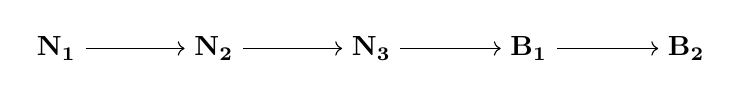
\begin{tikzpicture}
\node(a) at (7,0) {$\mathbf{N_{1}}$};
\node(b) at (9,0) {$\mathbf{N_{2}}$};
\node(c) at (11,0) {$\mathbf{N_{3}}$};
\node(d) at (13,0) {$\mathbf{B_{1}}$};
\node(e) at (15,0) {$\mathbf{B_{2}}$};

\draw[->] (a) -- (b);
\draw[->] (b) -- (c);
\draw[->] (c) -- (d);
\draw[->] (d) -- (e);
\end{tikzpicture}
\end{figure}

\noindent ただし$\mathbf{S_1}\longrightarrow\mathbf{S_2}$は,$\mathbf{S_1}$で導出可能な式がすべて$\mathbf{S_2}$でも導出可能であることを表す.

%この包含関係の列において,より左に位置するものはグラウンド理論的同値性に関してよりきめが細かく,より右に位置するものはよりきめが粗い.最もきめの粗い$\mathbf{B_{2}}$を見ると,この系のもとでのグラウンド理論的同値性は,内包的な同値性と近いきめの粗さを持っている.しかし$\mathbf{B_{2}}$は,吸収律 (A15, A16) を認めないという点で内包的な同値性よりもきめが細かい.一方で,最もきめの細かい$\mathbf{N_{1}}$のもとでのグラウンド理論的同値性は,構文的な同一性と近いきめの細かさを持っている.しかし$\mathbf{N_{1}}$は,交換律 (A1, A2) を認めるという点で構文的な同一性よりもきめが粗い.以上から,五つの公理系が要請RQを満たしていることが確かめられる.つまり,いずれの系も,少なくとも考慮に値するようなグラウンド理論的同値性の概念を規定しているということである\footnote{$\mathbf{B_{2}}$にA15, A16を加えると$\approx$は関連同値[relevant equivalence]と同等になり,さらにA17, A18を加えると実質同値と同等になる (cf. Correia\cite[p.265]{Correia2010}).}.

\subsection{いくつかの重要な規則}\label{notes}
上述の五つの体系は,グラウンド理論的同値性に関する規則の体系である.私たちはこれらに加えて,さらに四つのグラウンド ($\leq, <, \preceq, \prec$) に関する規則を立てることで,真理関数のためのグラウンドの非純粋な論理として十全なものを得ることができる.そのような規則として,すでに\textsc{PLG},導入規則,除去規則を私たちは検討した.さらにその他にも,いくつかの重要な非純粋な規則が存在する.Agglomeration, Convexity, Redundancy, Reduction Theoremである.本節の以下では,これらの規則がそれぞれ上のどの体系と整合的なのかを確かめる.以下で見る論点のいずれも,それぞれの体系の\emph{哲学的}解釈にかかわっているという意味で,グラウンドという哲学的概念のための論理体系を構築する試みにとって重要である.

%\subsubsection{冪等律A8, A9, A10と極大な命題}
%冪等律A8, A9, A10は\textsc{Basic Equivalences}の要素で,これを認めるかどうかが$\mathbf{N_{1}}, \mathbf{N_{2}}, \mathbf{N_{3}}$のグループと$\mathbf{B_{1}}, \mathbf{B_{2}}$のグループの間の主要な差異である.すでに見た通り,これら冪等律を認める一つの動機は,そうするとシンプルな導入規則\textsc{Introduction Rules}を妥当にできるということである.ここではそれとは別の,これらの規則を認めるないし認めない哲学的な動機があることを確認する.

%これらを認めない動機は,「あらゆる命題は\emph{何か}をグラウンドする」という原則にある (cf. Correia\cite{Correia2017}).たとえばA8を拒否すれば,(そしてそれに伴って二重否定の導入規則$\lnot\lnot$-I($<$)を認めれば)あらゆる命題はその二重否定を厳密にグラウンドすることが保証される.A9, A10を拒否する場合は,それぞれ,あらゆる命題がその自己連言,自己選言を厳密にグラウンドすることが保証される.それゆえ,この原則にもっともらしさを感じる者は,A8, A9, A10の少なくともいずれかを拒否するべきなのである.

%対して,A8, A9, A10を認める動機は,これとは対照的である.つまり,A8, A9, A10をすべて認めると,何もグラウンドしないような\emph{極大の}命題の存在が保証されるのである.(極大の命題とは,直観的には世界全体のあり方を表現しているような命題のことだと理解できよう.)この点はあまり明示的に論じられていないが,しかしA8, A9, A10を妥当にするFine\cite{Fine2016,Fine2017a,Fine2017b}の真理メーカー意味論においては,実際にそのような極大の命題が存在する.このような極大の命題の存在を認めたければ,A8, A9, A10を受け入れる必要がある.

\subsubsection{Agglomeration}\label{agglomeration}
まず,Agglomerationと呼ばれる次の規則を取り上げよう (cf. Lovett\cite{Lovett2020})\footnote{
AgglomerationはLovett\cite{Lovett2020}が提案している.ただし,Lovettは,$\lnot\lnot$-Agglomerationのかわりに,
\begin{prooftree}
\AxiomC{}
\LeftLabel{$\lnot\lnot$-Idempotence}
\UnaryInfC{$\lnot\lnot A\leq A$}
\end{prooftree}
を提案する.しかし,実はこれは$\lnot\lnot$-Agglomerationと同等である.(i) $\lnot\lnot$-Idempotenceを仮定する.$\lnot\lnot$-I($\leq$)より$A\leq\lnot\lnot A$であり,さらにDef($\approx$)から$\lnot\lnot A\approx A$である.するとSubstitution-Lより$\lnot\lnot$-Agglomerationが導出される.(ii) $\lnot\lnot$-Agglomerationを仮定する.弱いグラウンドの反射性より$A\leq A$であり,すると$\lnot\lnot$-Agglomerationから$\lnot\lnot A\leq A$が導かれる.
}.
\begin{itemize}
\item \textsc{Agglomeration}
\[
\begin{bprooftree}
	\AxiomC{$A, B, \Delta\leq C$}
	\LeftLabel{$\land$-Agglomeration}
	\UnaryInfC{$A\land B, \Delta\leq C$}
\end{bprooftree}
\qquad
\begin{bprooftree}
	\AxiomC{$A, \Delta\leq C$}
	\AxiomC{$B, \Gamma\leq C$}
	\LeftLabel{$\lor$-Agglomeration}
	\BinaryInfC{$A\lor B, \Delta, \Gamma\leq C$}
\end{bprooftree}
\]
\[
\begin{bprooftree}
	\AxiomC{$\lnot A, \Delta\leq C$}
	\AxiomC{$\lnot B, \Gamma\leq C$}
	\LeftLabel{$\lnot\land$-Agglomeration}
	\BinaryInfC{$\lnot(A\land B), \Delta, \Gamma\leq C$}
\end{bprooftree}
\qquad
\begin{bprooftree}
	\AxiomC{$\lnot A, \lnot B, \Delta\leq C$}
	\LeftLabel{$\lnot\lor$-Agglomeration}
	\UnaryInfC{$\lnot(A\lor B), \Delta\leq C$}
\end{bprooftree}
\]
\begin{prooftree}
	\AxiomC{$A, \Delta\leq C$}
	\LeftLabel{$\lnot\lnot$-Agglomeration}
	\UnaryInfC{$\lnot\lnot A, \Delta\leq C$}
\end{prooftree}
\end{itemize}

これらの規則は,弱いグラウンドの\emph{左側}に真理関数的に複雑な式を導入するための規則である.たとえば$\land$-Agglomerationは,$A, B$が$C$を弱くグラウンドするならば,$A\land B$も$C$を弱くグラウンドする,という規則である.これらの規則は,少なくとも一見したところは直観的である.また,弱いグラウンドの\emph{右側}の導入規則としての\textsc{Introduction Rules($\leq$)}に加えて,こうした左側の導入規則も立てることは,理論的な対称性をもたらしてくれる\footnote{Lovettはこの対称性に加え,さらにAgglomeration規則から$\mathbf{B_{2}}$の規則がすべて導出されることによって体系の単純性が得られるという事実が,これらの規則を受け入れるアブダクティブな理由を与えると論じている.また,\ref{iplg}節で詳しく見るが,他にも重要な規則がAgglomerationから導出される.}.この点でAgglomerationは理論的な美徳を持っていると言えよう.

さて,この\textsc{Agglomeration}は,しかし,上述の五つの体系のうち$\mathbf{N_{1}, N_{2}, N_{3}, B_{1}}$と不整合である.というのも,Lovett\cite[Appendix A.3]{Lovett2020}が示す通り,Def($\approx$)と\textsc{Introduction Rules($\leq$)}と\textsc{Agglomeration}から,$\mathbf{B_{2}}$に属する規則のうちR5以外の\emph{すべて}が導出可能だからである\footnote{
より特定的には,$\land$-AgglomerationがA1, A9, A11, R3を,$\lor$-AgglomerationがA2, A10, A12, R4を導出する.$\land$-Agglomerationと$\lor$-Agglomerationを合わせるとA6, A13, A14が導出される.$\lnot\land$-Agglomerationと$\lor$-Agglomerationを合わせるとA4が,$\lnot\lor$-Agglomerationと$\land$-Agglomerationを合わせるとA5が出る.$\lnot\lnot$-AgglomerationはA8, R6を導出し,これと$\lor$-Agglomerationを合わせるとA7を導出できる (Lovett\cite[Appendix A.3]{Lovett2020}).
}.それゆえ,仮に\textsc{Agglomeration}を認めたければ,グラウンド理論的同値性の体系としては$\mathbf{B_{2}}$をとる他ない.

ただし,\textsc{Agglomeration}は次のように弱めることが可能である.つまり,$\lor$-Agglomerationを次のものに置き換えるのである.

\begin{prooftree}
	\AxiomC{$A, \Delta\leq C$}
	\AxiomC{$B, \Delta\leq C$}
	\LeftLabel{Weak $\lor$-Agglomeration}
	\BinaryInfC{$A\lor B, \Delta\leq C$}
\end{prooftree}

\noindent Weak $\lor$-Agglomerationは,コンテクスト$\Delta$が左右の前提で同一であるように$\lor$-Agglomerationを制限した規則である.\textsc{Agglomeration}をこのように置き換えた規則の集合を\textsc{Weak Agglomeration}と呼ぶことにしよう.興味深いことに,\textsc{Weak Agglomeration}はA14を導出\emph{しない}ことをLovett\cite[pp.21-3]{Lovett2020}が示している.従って,\textsc{Weak Agglomeration}は$\mathbf{B_{2}}$だけでなく$\mathbf{B_{1}}$とも整合的である.(一方で,やはり$\mathbf{N_{1}, N_{2}, N_{3}}$とは不整合である.)
%
%
%
\subsubsection{Convexity,分配律 (A14),弱く部分的なグラウンド}\label{convexity}
続いて,Convexityと呼ばれる次の規則を検討しよう (cf. Kr\"{a}mer and Roski\cite{KramerandRoski2015}).

\begin{prooftree}
	\AxiomC{$\Gamma<C$}
	\AxiomC{$\Gamma, \Delta, E<C$}
	\LeftLabel{Convexity}
	\BinaryInfC{$\Gamma, \Delta<C$}
\end{prooftree}

\noindent この規則は,$\Gamma$と$\Gamma, \Delta, E$がどちらも$C$を厳密にグラウンドするとき,それらの「間」にある$\Gamma, \Delta$もまた$C$を厳密にグラウンドする,ということを許すものである.

以下では,この規則を認めない動機と認める動機を順に見ていく.まずは認めない動機から確認しよう.この規則は,グラウンドする命題とされる命題との間の\emph{関連性}にかかわる,とKr\"{a}mer and Roski\cite{KramerandRoski2015}が指摘している.特に,Convexityを仮定すると,
\begin{align*}
A, B<A\lor(B\land C)
\end{align*}
という形の式が導出されることが,関連性の観点から見ると問題をはらんでいるのである.問題の導出可能性に関するKr\"{a}mer and Roski\cite[pp.63--4]{KramerandRoski2015}の議論は次の通りである.

\begin{fact}
(補助的な仮定のもとで,)Convexityから$A, B<A\lor(B\land C)$が導出可能である.
\begin{proof}
まず,議論の一般性のため,前提つきの導入規則\textsc{Introduction Rules$^{*}(<)$}を仮定する.(前提つきの導入規則はグラウンド理論的同値性のどの体系とも整合的であるからである.)さらに,導入規則の前提を満たすために,
\begin{align*}
&B\land C\not\preceq A& &B\not\preceq C& &C\not\preceq B& &A\not\preceq B\land C
\end{align*}

\noindent がすべて成り立っていると仮定する.(この仮定はそれほど強いものではない.再び,相互に無関係であるような命題$A, B, C$を想定すればよい.)この仮定のもとで,問題の式は次のようにして導出される.
%仮定と$\lor$-I$_{1}^{*}(<)$から, $A<A\lor(B\land C)$である.同様に,仮定と$\lor$-I$_{1}^{*}(<)$, $\lor$-I$_{2}^{*}(<)$, $\land$-I$^{*}(<)$とCut($<$)から,$A, B, C<A\lor(B\land C)$である.これらにConvexityを適用すれば,$A, B<A\lor(B\land C)$が導出される.
まず,次の証明木を$\mathcal{D}$とする.

\begin{prooftree}
\AxiomC{$B\land C\not\preceq A$}
\LeftLabel{$\lor$-I$^{*}_{1}(<)$}
\UnaryInfC{$A<A\lor(B\land C)$}
	\AxiomC{$A\not\preceq B\land C$}
	\LeftLabel{$\lor$-I$^{*}_{2}(<)$}
	\UnaryInfC{$B\land C<A\lor(B\land C)$}
\LeftLabel{Amalgamation}
\BinaryInfC{$A, B\land C<A\lor(B\land C)$}
\end{prooftree}

その上で,所望の証明木は次の通りである.

\begin{prooftree}
\AxiomC{$B\land C\not\preceq A$}
\LeftLabel{$\lor$-I$^{*}_{1}(<)$}
\UnaryInfC{$A<A\lor(B\land C)$}
	\AxiomC{$B\not\preceq C$}
	\AxiomC{$C\not\preceq B$}
	\LeftLabel{$\land$-I$^{*}(<)$}
	\BinaryInfC{$B, C<B\land C$}
		\AxiomC{$\mathcal{D}$}
		\noLine
		\UnaryInfC{$A, B\land C<A\lor(B\land C)$}
	\LeftLabel{Cut$(<)$}
	\BinaryInfC{$A, B, C<A\lor(B\land C)$}
\LeftLabel{Convexity}
\BinaryInfC{$A, B<A\lor(B\land C)$}
\end{prooftree}

\end{proof}
\end{fact}

しかし,$A, B<A\lor(B\land C)$の何が問題なのか? これが問題であることを,Kr\"{a}mer and Roski\cite{KramerandRoski2015}は以下のように論じる.問題の要点は,このケースにおいて$B$が成り立つことは,$A\lor(B\land C)$が成り立つことをを説明するのに貢献し\emph{ない}ように思われるということである.このことは次のように理解されよう.$A$が成り立っているとすると,選言の真理条件から,$A\lor(B\land C)$も成り立つ.すると$A\lor(B\land C)$が成り立つのは$A$が成り立つおかげだと言える.対して,$B$だけが成り立っていても,$C$が成り立っていなければ$A\lor(B\land C)$は成り立たない.すると,$A\lor(B\land C)$が成り立っているのは$B$が成り立っているおかげではないように見える.つまり命題$A, B$の集合は,$B$がなくてもよいという意味で,$A\lor(B\land C)$にとって\emph{集合的な関連性}[collective relevance]を持たないのである (cf. Kr\"{a}mer and Roski\cite[p.65]{KramerandRoski2015}).ただしKr\"{a}mer and Roskiはやや譲歩して,$A, B$はそれぞれが個別に$A\lor(B\land C)$と関連しているという意味で,ここには\emph{分配的な関連性}[distributive relevance]があるとは言えるとも論じる.しかしKr\"{a}mer and Roskiは,「おかげである」という関係は,その直観的な理解からして集合的な関連性を満たすべきであり,そしてグラウンド関係はこの「おかげである」関係に他ならないのだから,グラウンドは集合的な関連性を満たすべきだと論じる.従って,この集合的な関連性を満たさない事例を帰結するConvexityは拒否されるべきだということになる.

また,興味深いことに,Convexityは分配律の片側のA14ともかかわっている.まず,上と同じ状況のもとで,A14からもまた$A, B<A\lor(B\land C)$が導出されてしまう (cf. Kr\"{a}mer and Roski\cite[pp.62--3]{KramerandRoski2015}, also cf. Correia\cite[pp.119-20]{Correia2016}).それゆえ,「集合的な関連性」の観点からConvexityに反対する者は,A14も拒否しなければならない.さらに,ConvexityとA14の間にはより直接的な結びつきもある.実は,(Kr\"{a}mer and Roski\cite{KramerandRoski2015}が示しているわけではないが,)適切な仮定のもとで,A14からConvexityが導出されるのである(証明は\ref{districonv}の事実\ref{a14con}を見よ).従って,いかなる理由であれ,Convexityを拒否するならばA14も拒否しなければならない.

以上が,Convexityを(それゆえA14を)認めない動機である.続いて,Convexityを認める動機に移ろう.Lovett\cite[p.23fn20]{Lovett2020}はそのような動機が存在することを,次のように示唆する.つまり,叙実的なグラウンドと非叙実的なグラウンドを区別すれば,問題の式の一見したところのもっともらしくなさは緩和されるかもしれないのである.Lovettはこれ以上のことを論じてはいないが,しかし上で見たKr\"{a}mer and Roskiの議論と接続すると,Lovettが言いたいのはおそらく次のようなことである.まず,\ref{factivenonfactive}節で見た通り,叙実的なグラウンドは実際に成り立っている命題の間を結ぶもので,これに対し非叙実的なグラウンドは単に可能な命題や不可能な命題の間をも結びうるものだということを思い起こそう.すると,たしかに,$A$と$B$が$A\lor(B\land C)$を叙実的にグラウンドすると言うのは奇妙かもしれない.なぜなら,$B$が\emph{実際に}成り立っていなくてもよいからである.しかし,$A$と$B$が$A\lor(B\land C)$を非叙実的にグラウンドすると言うことはそれほど奇妙ではないように思われる.というのも,$B$はたしかに$A\lor(B\land C)$が\emph{実際に}成り立つことを説明するのには貢献していないが,しかし,それが成り立ち\emph{うる}ことを説明するのには貢献しているからである.つまり,$A\lor(B\land C)$が成り立つことについて,それが$A$が成り立つおかげである可能性と,$B$(と$C$)が成り立つおかげである可能性の二つがあり,$B$はこの二つ目の可能性に貢献しているということである.(また,このことは,$A, B$が$A\lor(B\land C)$と分配的に関連している,ということの別の語り方だとも理解できよう.$A$は一つ目の可能性に個別に関連しており,$B$は二つ目の可能性に個別に関連しているのである.)

以上が,Convexityを認めない動機と認める動機である.いずれの動機にも一定の説得力があると私は思う.ここでさらに,別の関連する論点もとりあげよう.実は,ConvexityとA14は\emph{弱く部分的なグラウンド}の本性にもかかわっているのである.まず,弱く部分的なグラウンドは次のように定義されるのが自然だろう.
\begin{align}\label{def1}
A\preceq B \;\;\Leftrightarrow\;\; ある式Cが存在して,A, C\leq B.
\end{align}
この定義は,命題$A$が命題$B$を弱く部分的にグラウンドするというのは,$A$にある命題$C$を補うと$B$を弱く完全にグラウンドするのに十分だということだ,という考えを反映している.この定義は,本論冒頭で弱く部分的なグラウンドの概念を導入した際の特徴づけを率直に表現したものである.その上でLovett\cite{Lovett2020}は,A14を認めると,
\begin{align}\label{def2}
ある式Cが存在して,A, C\leq B \;\;\Leftrightarrow\;\; A, B\leq B.
\end{align}
が成り立つという興味深い事実を示している\footnote{
A14を認めると,
\begin{prooftree}
	\AxiomC{$A, \Delta\leq C$}
	\LeftLabel{Exchange}
	\UnaryInfC{$A, C\leq C$}
\end{prooftree}
という規則が導出可能であり,このExchangeによって(\ref{def2})が正当化されるのである.詳細はLovett\cite[pp.31--32]{Lovett2020}を見よ.
}
.すると (\ref{def1}), (\ref{def2})より,弱く部分的なグラウンドを次のように対象言語で定義することができる\footnote{このように\emph{規則の形で}弱く部分的なグラウンドを弱く完全なグラウンドによって定義できることは,弱く部分的なグラウンド$(\preceq)$はプリミティブなオペレーターとする必要がないということであり,従ってよりわずかな語彙のみを認めれば十分であることを意味する.(対して (\ref{def1}) の定義メタ言語でなされた量化的なものであるので,私たちの対象言語で表現することができない.)従ってA14を認めることは,論理体系の倹約性に貢献すると言える.}.

\begin{prooftree}
	\AxiomC{}
	\LeftLabel{Def($\preceq$)}
	\UnaryInfC{$A\preceq B\leftrightarrow A, B\leq B$}
\end{prooftree}

一方で,このDef($\preceq$)を認めると,再び問題の式$A, B<A\lor(B\land C)$が,上と同じ仮定のもと,次のようにして導出される.
\begin{fact}
Def($\preceq$)を仮定すると,(補助的な他の仮定のもとで)$A, B<A\lor(B\land C)$が導出可能である.
\begin{proof} 
次の式を仮定する.
\begin{align*}
&B\land C\not\preceq A& &B\not\preceq C& &C\not\preceq B& &A\not\preceq B\land C
\end{align*}

\noindent このとき,次のようにしてDef($\preceq$)から$A, B<A\lor(B\land C)$が導出される.

\scriptsize
\begin{prooftree}
\AxiomC{}
\LeftLabel{$\lor$-I$^{*}_{1}(<)$}
\UnaryInfC{$A\leq A\lor(B\land C)$}
	\AxiomC{$\vdots$}
	\UnaryInfC{$B, C<A\lor(B\land C)$}
	\LeftLabel{包摂$(</\prec)$}
	\UnaryInfC{$B\prec A\lor(B\land C)$}
	\LeftLabel{包摂$(\prec/\preceq)$}
	\UnaryInfC{$B\preceq A\lor(B\land C)$}
	\LeftLabel{Def$(\preceq)$}
	\UnaryInfC{$B, A\lor(B\land C)\preceq A\lor(B\land C)$}
\LeftLabel{Cut$(<)$}
\BinaryInfC{$A, B\leq A\lor(B\land C)$}
	\AxiomC{$\vdots$}
	\UnaryInfC{$A\prec A\lor(B\land C)$}
		\AxiomC{$\vdots$}
		\UnaryInfC{$B\prec A\lor(B\land C)$}
\LeftLabel{逆包摂}
\TrinaryInfC{$A, B<A\lor(B\land C)$}
\end{prooftree}
\normalsize

\end{proof}
\end{fact}
%$\lor$-I$_{2}^{*}(<)$, $\land$-I$^{*}(<)$とCut$(<)$から$B, C<A\lor(B\land C)$である.包摂($</\prec$)より$B\prec A\lor(B\land C)$,さらに包摂($\prec/\preceq$)より$B\preceq A\lor(B\land C)$である.するとDef($\preceq$)より,$B, A\lor(B\land C)\leq A\lor(B\land C)$である.また,これと$A<A\lor(B\land C)$,包摂($</\leq$),Cut$(\leq)$より,$A, B\leq A\lor(B\land C)$.いま,$A\prec A\lor(B\land C), B\prec A\lor(B\land C)$であるから,逆包摂より$A, B<A\lor(B\land C)$が導出される.

\noindent 従って,「集合的な関連性」の観点からConvexityやA14を拒否する者は,同じ理由でDef($\preceq$)も拒否しなければならない.それゆえ,そのような見解に立つものは,弱く部分的なグラウンドの定義としては(\ref{def1})を利用する必要がある.さらに,Def($\preceq$)とConvexity, A14との間には,再び,より直接的な関係がある.適切な仮定のもとで,Def$(\preceq)$からConvexityとA14が導出されるのである(\ref{districonv}の事実\ref{defcon},\ref{defa14}を見よ).従って,一般に,ConvexityやA14を拒否するならばDef$(\preceq)$も拒否しなければならず,それゆえ弱く部分的なグラウンドの定義としては(\ref{def1})を利用する必要があるのである.

ここで,$\mathbf{N_{1}, N_{2}, N_{3}, B_{1}}$と$\mathbf{B_{2}}$はA14を認めるかどうかで対立していることを思い起こそう.すると,A14を認める$\mathbf{B_{2}}$はDef($\preceq$)と整合的だが,A14を認めない$\mathbf{N_{1}, N_{2}, N_{3}, B_{1}}$はそうではないということになる.すなわち,$\mathbf{N_{1}, N_{2}, N_{3}, B_{1}}$と$\mathbf{B_{2}}$では弱く部分的なグラウンドの定義が異なるのである.このことは,それらの体系の間の興味深い,実質的な違いである.
%
%
%
\subsubsection{Redundancy,弱く完全なグラウンド,Reduction Theorem}\label{redundancy}
最後に,次のRedundancy規則 (cf. Correia\cite{Correia2017}, Kr\"{a}mer\cite{Kramer2018,Kramer2021}) に関する議論を見よう.

\begin{prooftree}
	\AxiomC{$\Gamma, C\leq C$}
	\LeftLabel{Redundancy}
	\UnaryInfC{$\Gamma\leq C$}
\end{prooftree}

\noindent この規則は,弱く完全なグラウンドを表す式において,「余分な」基本式(すなわち$C$)を取り除くことを許すものである.これは,先に見たConvexityとはまた異なる仕方で,グラウンドする命題とされる命題との間の関連性を規定する規則だと解釈できるだろう.

以下,Redundancyがどのような規則と不整合で,どのような規則と整合的であるのかを検討する.まず,Redundancyは\textsc{Weak Agglomeration}と整合的でない体系,つまり$\mathbf{N_{1}}, \mathbf{N_{2}}, \mathbf{N_{3}}$とは整合的であることが分かっている.(この事実は意味論的に確かめられる.そのため,証明論のみに注目する本論では取り扱うことができない.詳しくはCorreia\cite[p.525]{Correia2017}, Kr\"{a}mer\cite[p.1671]{Kramer2021}を見よ.本論脚注22も参照.)

一方で,Redundancyは,\textsc{Weak Agglomeration}と不整合である.特に,連言的な性格を持つ$\land$-Agglomerationと$\lnot\lor$-Agglomerationが問題となる.

\begin{fact}\label{redwe}
Redundancyと\textsc{Weak Agglomeration}は不整合である
\begin{proof}
Redundancyと$\land$-Agglomerationが不整合であることを示す.まず,
\begin{align*}
B\not\preceq A
\end{align*}
であるような状況を想定しよう.(直観的な解釈としては,やはり相互に無関係であるような二つの命題$A, B$を考えればよい.ここでは〈りんごが存在する〉と〈風船が存在する〉とする.)すると,次のようにして$A\leq A\land B$が導出される.

\begin{prooftree}
\AxiomC{}
\LeftLabel{$\land$-I($\leq$)}
\UnaryInfC{$A, B\leq A\land B$}
\LeftLabel{Repetition}
\UnaryInfC{$A, A, B\leq A\land B$}
\LeftLabel{$\land$-Agglomeration}
\UnaryInfC{$A, A\land B\leq A\land B$}
\LeftLabel{Redundancy}
\UnaryInfC{$A\leq A\land B$}
\end{prooftree}

\noindent 結論の$A\leq A\land B$は現在の解釈だと,〈りんごが存在する〉が〈りんごと風船が存在する〉を弱く完全にグラウンドする,ということである.しかし,〈りんごが存在する〉の説明上の役割は,風船に関する情報を含まず,従って〈りんごと風船が存在する〉の説明上の役割を包摂しないだろう.よってこの結論は認めるべきではない.
\end{proof}
\end{fact}

それゆえ,$\land$-Agglomerationと$\lnot\lor$-Agglomerationを認めるならばRedundancyを認めるべきではない.従って,\textsc{Weak Agglomeration}と整合的な$\mathbf{B_{1}, B_{2}}$のもとでは,Redundanryを拒否するのが自然だと言える.

以上が,Redundancyと他の規則との間の整合性に関する事実である.このRedundancyを妥当だと見なすべきか否かについての哲学的な議論は,未だ精力的にはなされておらず,この点は今後の課題として残されている.さて,本節の最後に,関連する別の論点を提示しておこう.実は,Redundancyは\emph{弱く完全なグラウンド}の本性にかかわっているのである.Redundancyと整合的な$\mathbf{N_{1}}, \mathbf{N_{2}}, \mathbf{N_{3}}$では,弱いグラウンドを次の命題によって特徴づけることができる (cf. Correia\cite[p.530]{Correia2017}, Kr\"{a}mer\cite[pp.1649--50]{Kramer2021}).

\begin{align}\label{def3}
&\Gamma\leq C \;\;\Leftrightarrow\notag\\
&\;\;\text{(i)}\;\Gamma\approx C \;\;または,\notag\\
&\;\;\text{(ii)}\;\Gamma<C \;\;または,\notag\\
&\;\;\text{(iii)}\;\Gamma_1\cup\Gamma_2=\Gamma なる\Gamma_1, \Gamma_2 が存在して,\Gamma_1\approx C かつ \Gamma_2<C.
\end{align}

\noindent ただし「$\Gamma\approx C$」は,「すべての$A\in\Gamma$について$A\approx C$」の略記である.実際,(\ref{def3}) はRedundancyを含意することをCorreia\cite[p.525]{Correia2017},Kr\"{a}mer\cite[p.803]{Kramer2018}が示している.さらにその逆,つまりRedundancyが (\ref{def3}) を含意することも示せる(証明は\ref{representational}の事実\ref{reddefleq}を見よ).従って (\ref{def3}) とRedundancyは同等である.

それゆえ,\textsc{Weak Agglomeration}を認める(従ってRedundancyを認めない)場合,弱く完全なグラウンドは別の仕方で特徴づけられなければならない.具体的には,弱く完全なグラウンドはグラウンド理論的同値性によって,次のようにして対象言語で特徴づけられることになる\footnote{
弱いグラウンドのこのような特徴づけは,グラウンドの論理の初期の研究であるCorreia\cite{Correia2010}に由来する.ただしCorreiaはそれを「弱いグラウンド」ではなく「選言的包含[disjunctive containment]」と呼び,「$A$が$B$を選言的に包含する」を「$A\geq^{d}B$」と書く.$A\geq^{d}B$と$B\leq A$は同じことを述べている.
} (cf. Lovett\cite{Lovett2020}).

\begin{prooftree}
	\AxiomC{}
	\LeftLabel{Reduction Theorem$(\leq/\approx)$}
	\UnaryInfC{$\Delta\leq B\leftrightarrow B\approx B\lor\widehat{\Delta}$}
\end{prooftree}

\noindent ただし$\widehat{\Delta}$は,$\Delta$に属する式すべてを,左から順に連言で結んだものである\footnote{Reduction Theoremは,Def($\approx$), $\land$-Agglomeration, そしてWeak $\lor$-Agglomerationを仮定すると導出可能である(証明はLovett\cite[p.27]{Lovett2020}を見よ).}.このReduction Theoremは,Redundancyと不整合である.
\begin{fact}\label{redred}
Reduction TheoremとRedundancyは不整合である.

\begin{proof}
Reduction TheoremとRedundancyを仮定すると,次のようにして$A\leq A\land B$が導出可能である.しかし,この式は事実\ref{redwe}でも問題視されたものだった.

\footnotesize
\begin{prooftree}
\AxiomC{}
\LeftLabel{A10}
\UnaryInfC{$A\land B\approx(A\land B)\lor(A\land B)$}
	\AxiomC{}
	\LeftLabel{A9}
	\UnaryInfC{$A\approx A\land A$}
	\LeftLabel{R3}
	\UnaryInfC{$A\land B\approx(A\land A)\land B$}
		\AxiomC{}
		\LeftLabel{A11}
		\UnaryInfC{$(A\land A)\land B\approx A\land(A\land B)$}
	\LeftLabel{R2}
	\BinaryInfC{$A\land B\approx A\land(A\land B)$}
	\LeftLabel{R4}
	\UnaryInfC{$(A\land B)\lor(A\land B)\approx A\land(A\land B)\lor(A\land B)$}
\LeftLabel{R2}
\BinaryInfC{$A\land B\approx A\land(A\land B)\lor(A\land B)$}
\LeftLabel{Reduction Theorem}
\UnaryInfC{$A, A\land B\leq A\land B$}
\LeftLabel{Redundancy}
\UnaryInfC{$A\leq A\land B$}
\end{prooftree}
\normalsize
\end{proof}
\end{fact}

\noindent 従って,Reduction Theoremによる弱く部分的なグラウンドの特徴づけは,Redundancyと同等な (\ref{def3}) による特徴づけと不整合である.

以上から,\textsc{Weak Agglomeration}を基準として,$\mathbf{B_{1}}, \mathbf{B_{2}}$のグループと$\mathbf{N_{1}}, \mathbf{N_{2}}, \mathbf{N_{3}}$のグループの間で弱く完全なグラウンドの特徴づけが異なるということが分かる.このことは,それらの体系の間の実質的な違いである.

さて,本節では,グラウンド理論的同値性のための五つの体系を提示し,それらを比較した.また,Agglomeration, Convexity, Redundancy, Reduction Theoremなど,いくつかの興味深い規則が存在することが確かめられた.これらの規則はいずれも,弱く部分的なグラウンド,弱く完全なグラウンドの定義の仕方に影響するという点で,グラウンドの論理にとって本質的に重要である.次節ではこうした検討を踏まえ,真理関数のためのグラウンドの非純粋な論理として提案されているいくつかの体系を要約する.
%
%
%
\section{真理関数のためのグラウンドの非純粋な論理}\label{iplg}
ここまでで,真理関数,四種類のグラウンド,そしてグラウンド理論的同値性が相互に関連する仕方を検討してきた.本節では以上の考察を合わせて,真理関数のためのグラウンドの非純粋な論理が,全体としてはどのような規則から構成されることになるのかを見る.残念ながら,$\mathbf{N_{2}, N_{3}, B_{1}}$をベースにした非純粋な論理は,いまだ十全なものは提案されていない\footnote{示唆的な仕事としてはKr\"{a}mer\cite{Kramer2018,Kramer2021}, Correia\cite{Correia2016}を見よ.}.それゆえ,この点で本節の記述は断片的なものにならざるをえない.しかしながら,幸いにして$\mathbf{N_{1}, B_{2}}$をベースにした非純粋な論理としては,すでに十全な形で提案された体系が存在する.$\mathbf{B_{2}}$の拡張としての$\mathbf{B_{2}^{+}}$と$\mathbf{B_{2}^{+f}}$,$\mathbf{N_{1}}$の拡張としての$\mathbf{N_{1}^{+}}$である.それらは表\ref{ImpureLogics}のように整理される.本節ではこれらの体系を順番に要約する.

\begin{table}[h]
\caption{非純粋な論理の比較}
\label{ImpureLogics}
\centering
	\begin{tabular}{cccc}
	\hline
	 & $\mathbf{B_{2}^{+}}$ & $\mathbf{B_{2}^{+f}}$ & $\mathbf{N_{1}^{+}}$ \\
	\hline \hline
	叙実的/非叙実的 & 非叙実的 & 叙実的 & 非叙実的 \\
	導入規則 & \textsc{Intr. Rules$^{*}(<)$} & \textsc{Intr. Rules$^{*}(<)$} & \textsc{Intr. Rules$(<)$} \\
	除去規則 & \textsc{Elim. Rule$^{*}(<)$} & \textsc{Elim. Rule$^{*}(<)$} & \textsc{Elim. Rule$(<)$} \\
	Convexity & 妥当 & 妥当 & 非妥当 \\
	Agglomeration & 妥当 & 妥当 & 非妥当 \\
	Reduction Theorem & 妥当 & 妥当 & 非妥当 \\
	Redundancy & 非妥当 & 非妥当 & 妥当 \\
	\hline
	\end{tabular}
\end{table}

\subsection{$\mathbf{B_{2}}$の非純粋な拡張$\mathbf{B_{2}^{+}}$}
$\mathbf{B_{2}}$の規則をすべて妥当にするような非純粋な体系$\mathbf{B_{2}^{+}}$は,Lovett\cite{Lovett2020}が示している.その体系は次の規則からなる.
\begin{itemize}
\item \textsc{Defs}($\mathbf{B_{2}^{+}}$)
\[
\begin{bprooftree}
\AxiomC{}
\LeftLabel{Def($\preceq$)}
\UnaryInfC{$A\preceq B\leftrightarrow A, B\leq B$}
\end{bprooftree}
\qquad
\begin{bprooftree}
\AxiomC{}
\LeftLabel{Def($\prec$)}
\UnaryInfC{$A\prec B\leftrightarrow A\preceq B\land B\not\preceq A$}
\end{bprooftree}
\]

\begin{prooftree}
\AxiomC{}
\LeftLabel{Def($<$)}
\UnaryInfC{$A_1, A_2, \ldots<B\leftrightarrow(A_1, A_2, \ldots\leq B)\land(B\not\preceq A_1)\land(B\not\preceq A_2)\land\ldots$}
\end{prooftree}

\begin{prooftree}
	\AxiomC{}
\LeftLabel{Def($\approx$)}
	\UnaryInfC{$A\approx B\leftrightarrow A\leq B\land B\leq A$}
\end{prooftree}

\item \textsc{The Pure Logic of Ground}($\mathbf{B_{2}^{+}}$)
\begin{prooftree}
	\AxiomC{$\Delta_1\leq A_1$}
	\AxiomC{$\Delta_2\leq A_2$}
	\AxiomC{$\ldots$}
	\AxiomC{$A_1, A_2, \ldots\leq C$}
\LeftLabel{Cut($\leq$)}
	\QuaternaryInfC{$\Delta_1, \Delta_2, \ldots\leq C$}
\end{prooftree}

\[
\begin{bprooftree}
	\AxiomC{}
\LeftLabel{同一性($\leq$)}
	\UnaryInfC{$A\leq A$}
\end{bprooftree}
\qquad
\begin{bprooftree}
	\AxiomC{$A$}
	\AxiomC{$A\leq B$}
\LeftLabel{IMP}
	\BinaryInfC{$B$}
\end{bprooftree}
\]

\item \textsc{The Impure Logic of Ground}($\mathbf{B_{2}^{+}}$)
\begin{align*}
\textsc{Introduction Rules($\leq$)} + \textsc{Agglomeration} + 
\end{align*}
\begin{prooftree}
	\AxiomC{$A\approx B$}
	\LeftLabel{A5}
	\UnaryInfC{$\lnot A\approx\lnot B$}
\end{prooftree}
\end{itemize}

\textsc{Defs}($\mathbf{B_{2}^{+}}$)によって,弱く完全なグラウンドから,それ以外の四つのオペレーターが定義される.\textsc{The Pure Logic of Ground}($\mathbf{B_{2}^{+}}$)は,すでに見たCut($\leq$)と同一性$(\leq)$に加え,グラウンドが真理保存的であることを保証する規則IMPからなる.\textsc{The Impure Logic of Ground}($\mathbf{B_{2}^{+}}$)は弱いグラウンドの左右の導入規則とA5からなる.この$\mathbf{B_{2}^{+}}$において,\ref{plg}節の\textsc{PLG}の規則,$\mathbf{B_{2}}$の規則,厳密なグラウンドの導入規則 (\textsc{Introduciton Rules$^{*}(<)$}) と除去規則 (\textsc{Elimination Rule$^{*}(<)$}) などが\emph{すべて}導出される.(証明はLovett\cite{Lovett2020}を参照.)

この体系の最大の特徴は,その単純さである.四つの定義とわずかな純粋な規則,そして弱く完全なグラウンドの左右の導入規則によって,大半の重要な規則が導出されるのである\footnote{A5のみがややアドホックに見える.しかし,実は$\mathbf{B_{2}}$からA5だけを落とした体系において,A5が許容可能な規則であることをFine\cite{Fine2016}が証明している.このことをを考えると,A5をプリミティブな規則として認めることにも十分な正当性があるように思われる.}.その結果,多くの規則の妥当性が$\mathbf{B_{2}^{+}}$の規則の妥当性から説明されることになる.Lovettはこの点に「説明上の美徳」があると強調する (Lovett\cite[p.32]{Lovett2020}).また,弱く完全なグラウンドのみがプリミティブであり,それから定義によって他の概念(弱く部分的なグラウンド,厳密で完全なグラウンド,厳密で部分的なグラウンド,グラウンド理論的同値)がすべて定義されることは,この体系の概念的な倹約性を示している.

また,この体系ではA14とConvexityが妥当である.よって,\ref{convexity}節で検討した通り,グラウンドは「分配的な関連性」を満たすだけでよく,必ずしも「集合的な関連性」を満たす必要はないというようにグラウンドを解釈するなら,この体系$\mathbf{B_{2}^{+}}$を採用するのが合理的である.また,弱く部分的なグラウンドはDef$(\preceq)$によって定義される.さらに,Def($\approx$)と\textsc{Agglomeration}のおかげでReduction Theoremが導出され,よって事実\ref{redred}よりRedundancyは非妥当である.すなわち,この体系では弱く完全なグラウンドはReduction Theoremによって特徴づけられることになる.
%
%
%
\subsubsection{叙実的なグラウンド:$\mathbf{G}$と$\mathbf{B_{2}^{+f}}$}
さらに,$\mathbf{B_{2}}$の規則を妥当にする\emph{叙実的な}体系として,Correia\cite{Correia2010}が$\mathbf{G}$と呼ばれる体系を提案している.(直前で見た$\mathbf{B_{2}^{+}}$は\emph{非叙実的な}体系である.)$\mathbf{G}$は,グラウンド理論的同値性オペレーターと,\emph{叙実的で}厳密で完全なグラウンドを表すオペレーター ($<_{f}$) のみを含む体系である.それゆえ,私たちは式の定義に次を追加する必要がある.
	\begin{itemize}
	\item[--] $\Gamma$が基本式の集合で$A$が基本式なら,$(\Gamma<_{f}A)$は式である.
	\end{itemize}
その上で体系$\mathbf{G}$は,グラウンド理論的同値性の体系$\mathbf{B_{2}}$を,次の定義によって叙実的なグラウンドに拡張したものである (cf. Correia\cite{Correia2010}, Lovett\cite{Lovett2020}).

\begin{prooftree}
\AxiomC{}
\LeftLabel{Def($<_{f}/\approx$)}
\UnaryInfC{$\Delta<_{f}B\leftrightarrow\widehat{\Delta}\land(B\approx B\lor\widehat{\Delta})\land(\Delta\not\approx\Delta\lor(B\land\Delta))$}
\end{prooftree}

\noindent ただし$\Delta\not\approx\Delta\lor(B\land\Delta)$は,$\Delta$のどの要素$C$についても$C\not\approx C\lor(B\land C)$であることを表す\footnote{私たちの言語でより正確に表現すると,これは長い連言になる.ここでは煩雑さを避けるため,このような省略的な記法を認めることにする.}.右辺の一つ目の連言肢$\widehat{\Delta}$は,「$\Delta$に属する式がすべて真である」という叙実性の条件を述べている.二つ目の連言肢は,(Reduction Theoremを仮定すれば)$\Delta\leq B$と同値である.三つ目の連言肢は,Reduction Theorem,  \textsc{Defs}($\mathbf{B_{2}^{+}}$), A14, A9を仮定すると,実は「$\Delta$のすべての要素$C$について,$B\not\preceq C$」と同値である.これが成り立つのは,
\begin{prooftree}
\AxiomC{}
\LeftLabel{Def$(\preceq/\approx)$}
\UnaryInfC{$B\preceq C\leftrightarrow C\approx C\lor(B\land C)$}
\end{prooftree}
という規則\footnote{
Correia\cite{Correia2010}は,$C\approx C\lor(B\land C)$として特徴づけられる$B, C$間の関係を,「弱く部分的なグラウンド」ではなく「選言的包含の連言的包含[conjunctive containment of disjunctive containment]」と呼び,「$C\geq^{cd}B$」と書く.$B\prec C$と$C\geq^{cd}B$は同じことを述べている.
}が,Def($\preceq$)とReduction Theorem,さらにA14, A9から導出されるからである (cf. Lovett\cite{Lovett2020}).従って,Def($<_{f}/\approx$)が述べているのは結局のところ,
\begin{align*}
&\Delta がBを\emph{叙実的に}厳密に完全にグラウンドする \;\Leftrightarrow \\
&\;\text{(i)}\;\Delta の要素がすべてが真で,かつ\\
&\;\text{(ii)}\;\Delta がBを弱く完全にグラウンドし,かつ\\
&\;\text{(iii)}\;Bが\Delta のどの要素も弱く部分的にグラウンドしない,
\end{align*}
ということである.そしてこの同値言明の右辺は,
\begin{align*}
\Delta の要素がすべてが真で,かつ\Delta がBを厳密に完全にグラウンドする,
\end{align*}
ということである.これを叙実的なグラウンドの定義とすることに異論はないだろう.

また,興味深いことに,$\mathbf{G}$にReduction Theoremと\textsc{Defs}($\mathbf{B_{2}^{+}}$)を追加した系$\mathbf{G^{*}}$と,$\mathbf{B_{2}^{+}}$にDef($<_{f}/\approx$)を追加した系$\mathbf{B_{2}^{+f}}$が同値であることをLovett\cite{Lovett2020}が示している.すなわち,
\begin{align*}
\mathbf{G^{*}} &= \mathbf{B_{2}} + \text{Reduction Theorem} + \textsc{Defs}(\mathbf{B_{2}^{+}}) + \text{Def}(<_{f}/\approx)\\
\mathbf{B_{2}^{+f}} &= \mathbf{B_{2}^{+}} + \text{Def}(<_{f}/\approx)
\end{align*}
なる二つの系が同値だということである.(それゆえ,当然$\mathbf{B_{2}} + \text{Reduction Theorem} + \textsc{Defs}(\mathbf{B_{2}^{+}})$と$\mathbf{B_{2}^{+}}$も同値である.)このことは,$\mathbf{G^{*}}$においても,$\mathbf{B_{2}^{+}}$で導出される重要な規則(PLGの規則や,前提つきの導入規則・除去規則など)が導出可能だということを意味する.すなわち,$\mathbf{G^{*}}$はたしかに$\mathbf{B_{2}^{+}}$の叙実的なバージョンだと言うことができる.

補足として,非叙実的な体系を叙実的な体系に拡張する一般的な方法を改めて述べ直しておこう.つまり,任意の非叙実的な体系に,
\begin{prooftree}
\AxiomC{}
\LeftLabel{Def($<_{f}/<$)}
\UnaryInfC{$\Delta<_{f}B\leftrightarrow\widehat{\Delta}\land(\Delta<B)$}
\end{prooftree}
という規則を追加することによって,その体系の叙実的なバージョンを得ることができるのである.あるいは,上と同じように,A14が妥当であるときは代わりにDef($<_{f}/\approx$)を追加することによっても同じ結果が得られる.
%
%
%
\subsection{$\mathbf{N_{1}}$の非純粋な拡張$\mathbf{N_{1}^{+}}$}
最後に,$\mathbf{N_{1}}$の規則をすべて妥当にする非純粋な体系を要約する.すでに,Correia\cite{Correia2017}がそのような体系を提案している.しかし,Correiaが構築するのは,(おそらく意味論的な単純さのために,)部分的なグラウンド ($\prec, \preceq$) を除外した,完全なグラウンド ($<, \leq$) とグラウンド理論的同値性 ($\approx$) のみのための体系である.その体系を$\mathbf{C}$と呼ぶことにしよう.ここでは,上の$\mathbf{B_{2}^{+}}, \mathbf{B_{2}^{+f}}$との比較のしやすさを考慮して,$\mathbf{C}$とは異なる,部分的なグラウンドも組み入れた体系$\mathbf{N_{1}^{+}}$を示す.(ただし,$\mathbf{C}$を定義によって部分的なグラウンドにも拡張した体系$\mathbf{C^{*}}$は,実は$\mathbf{N_{1}^{+}}$と同等である.証明は\ref{representational}を見よ.)

$\mathbf{N_{1}^{+}}$は以下の規則からなる体系である.
\begin{itemize}
\item \textsc{Defs}($\mathbf{N_{1}^{+}}$)
\begin{align*}
\textsc{Defs}(\mathbf{B_{2}^{+}}) - \text{Def}(\preceq)
\end{align*}

\item \textsc{The Pure Logic of Ground}($\mathbf{N_{1}^{+}}$)
\begin{align*}
\textsc{The Pure Logic of Ground}(\mathbf{B_{2}^{+}}) + 
\end{align*}

\[
\begin{bprooftree}
	\AxiomC{$\Delta, A\leq C$}
\LeftLabel{包摂($\leq/\preceq$)}
	\UnaryInfC{$A\preceq C$}
\end{bprooftree}
\qquad
\begin{bprooftree}
	\AxiomC{$A\preceq B$}
	\AxiomC{$B\preceq C$}
\LeftLabel{推移性($\preceq/\preceq$)}
	\BinaryInfC{$A\preceq C$}
\end{bprooftree}
\]

\[
\begin{bprooftree}
	\AxiomC{$A\prec B$}
	\AxiomC{$B\preceq C$}
\LeftLabel{推移性($\prec/\preceq$)}
	\BinaryInfC{$A\prec C$}
\end{bprooftree}
\qquad
\begin{bprooftree}
	\AxiomC{$A\preceq B$}
	\AxiomC{$B\prec C$}
\LeftLabel{推移性($\preceq/\prec$)}
	\BinaryInfC{$A\prec C$}
\end{bprooftree}
\]

\[
\begin{bprooftree}
\AxiomC{$A\preceq B$}
\AxiomC{$B\preceq A$}
\LeftLabel{反対称性}
\BinaryInfC{$A\approx B$}
\end{bprooftree}
\qquad
\begin{bprooftree}
\AxiomC{$\Gamma, A\leq A$}
\LeftLabel{Redundancy($\leq$)}
\UnaryInfC{$\Gamma\leq A$}
\end{bprooftree}
\]

\item \textsc{The Impure Logic of Ground}($\mathbf{N_{1}^{+}}$)
\begin{align*}
\mathbf{N_{1}} + \textsc{Introduction Rules($<$)} + \textsc{Elimination Rules($<$)} + 
\end{align*}

\begin{prooftree}
\AxiomC{$\Gamma, A<p$}
\LeftLabel{Complexity}
\RightLabel{\;\;\;(ただし$p$は文記号,$A$はそうでない)}
\UnaryInfC{$\bot$}
\end{prooftree}

\begin{prooftree}
\AxiomC{$A\approx B\land C$}
\LeftLabel{Complexity($\land$)}
\RightLabel{\;\;\;(ただし$A$の主結合子は$\land$ではない)}
\UnaryInfC{$\bot$}
\end{prooftree}

\begin{prooftree}
\AxiomC{$A\approx B\lor C$}
\LeftLabel{Complexity($\lor$)}
\RightLabel{\;\;\;(ただし$A$の主結合子は$\lor$ではない)}
\UnaryInfC{$\bot$}
\end{prooftree}

\begin{prooftree}
\AxiomC{$A\approx\lnot B$}
\LeftLabel{Complexity($\lnot$)}
\RightLabel{\;\;\;(ただし$A$の主結合子は$\lnot$ではない)}
\UnaryInfC{$\bot$}
\end{prooftree}

\begin{prooftree}
\AxiomC{$A\land B\approx A'\land B'$}
\LeftLabel{$\land$-E($\approx$)}
\UnaryInfC{$(A\approx A'\land B\approx B')\lor(A\approx B'\land B\approx A')$}
\end{prooftree}

\begin{prooftree}
\AxiomC{$A\lor B\approx A'\lor B'$}
\LeftLabel{$\lor$-E($\approx$)}
\UnaryInfC{$(A\approx A'\land B\approx B')\lor(A\approx B'\land B\approx A')$}
\end{prooftree}

\begin{prooftree}
\AxiomC{$\lnot A\approx\lnot B$}
\LeftLabel{$\lnot$-E($\approx$)}
\UnaryInfC{$A\approx B$}
\end{prooftree}
\end{itemize}
\textsc{Defs}($\mathbf{N_{1}^{+}}$)は,\textsc{Defs}($\mathbf{B_{2}^{+}}$)からDef$(\preceq)$を除いたものである.これを除かなければならないのは,\ref{convexity}節での検討から,A14を認めない$\mathbf{N_{1}}$とDef$(\preceq)$が不整合であるからである.また,それに伴い,純粋な規則として弱く部分的なグラウンドに関する包摂規則,推移性規則,反対称性規則を追加する必要が生じている\footnote{
反対称性規則が$\mathbf{B_{2}^{+}}$で導出可能かどうかは明らかではない.一方で,$\mathbf{C}$に対してCorreiaが与えている健全で完全な意味論では,反対称性規則が妥当になることが示されている (cf. Correia\cite{Correia2017}).よって$\mathbf{N_{1}^{+}}$ではこの規則を立てるべきである.
}.さらに,$\mathbf{N_{1}}$と整合的なRedundancyもプリミティブな規則として認めている.非純粋な規則としては,$\mathbf{N_{1}}$に加えて,無前提の導入規則・除去規則を立てる.さらに,新たに七つの規則もプリミティブな規則として採用している.

$\mathbf{N_{1}^{+}}$の一つの特徴的な点は,この七つの規則にある.これらの規則は合わせて,グラウンド理論的に同値であるような二つの式は,\emph{よく似た構文的構造}を持たなければならない,という制約を述べたものだと解釈できる.ただし,$\mathbf{N_{1}^{+}}$は規則A1とA2を認めているために,$A\land B$と$B\land A$,あるいは$A\lor B$と$B\lor A$は区別しない.従って正確に言えば,「よく似た」というのは,連言ないし選言で結ぶ順番の差異以外の構文的な構造には鋭敏だということである.

もう一つの特徴は,体系の複雑さである.\ref{gte}節で見た通り,この体系ではA14が妥当でないため,Def($\preceq$)を認めることができない.従って,弱く部分的なグラウンドはプリミティブなオペレーターとして扱う必要があり,それに伴い弱く部分的なグラウンドに関する包摂規則,推移性規則,反対称性規則を追加する必要が生じている.それゆえ,この$\mathbf{N_{1}^{+}}$は,$\mathbf{B_{2}^{+}}$よりも単純さの点で劣っている.しかしこのことは,Convexityが非妥当になるということの裏返しである.\ref{gte}節で見た「集合的な関連性」をグラウンドが持つべきだと考える動機が,理論の単純さを望む動機よりも強いのならば,この点はむしろ一つの長所と見られるべきだろう.

また,この体系ではRedundancyをプリミティブな規則としており,従って事実\ref{redred}よりReduction Theoremは非妥当である.それゆえ弱く完全なグラウンドは,\ref{redundancy}節で見たような仕方で,(\ref{def3}) によって特徴づけられることになる.すなわち,$\mathbf{N_{1}^{+}}$では弱く完全なグラウンドの特徴づけが$\mathbf{B_{2}^{+}}$におけるものとは異なる.この点もまた,$\mathbf{N_{1}^{+}}$と$\mathbf{B_{2}^{+}}$の間の本質的な差異だと言える.
%
%
%
\section{おわりに}
本論では,グラウンドの論理の研究状況をサーベイした.グラウンドの純粋な論理と非純粋な論理が区別され,前者はグラウンドそれ自体が持つ形式的特徴に,後者はグラウンドと論理演算子(本論では特に真理関数)との間の関係にかかわるものであった.また,グラウンド理論的同値性という概念が重要な役割を持っていることが確かめられた.すなわち,第一に,何と何がグラウンド理論的に同値で,何と何がそうでないと想定するかによって,真理関数に関する導入規則,除去規則としてどのような形のものを受け入れるべきであるかが決定されるのであった.そして第二に,導入規則,除去規則の他にも重要な規則が存在し,やはりそれらを受け入れるべきか否かという点でグラウンド理論的同値性の概念が本質的に重要だった.最後の節では,こうした考慮のもとで,真理関数のためのグラウンドの非純粋な論理として実際に提案されている三つの体系が要約・比較された.

さて,この第二の点の重要な規則として,Agglomeration, Convexity, Reduction Theorem, Redundancyといったものが存在することを私たちは見た.本論の成果は,これらの規則が他のどのような規則と整合的で,どれとそうではないのかを明確にした点にある.一方で,今後の展望として残されている問題もある.つまり,これらの規則を哲学的に解釈することである.今後の研究次第では,たとえばConvexityを正当化するようないかなる哲学的解釈も存在せず,従ってConvexityを妥当にする体系は拒否されるべきだと分かるかもしれない.あるいは,しかじかの目的にとってはConvexityを認める体系が適切であり,また別の目的にとっては別の体系が適切である,ということが分かるかもしれない.いずれにせよ,上記の興味深い規則の哲学的解釈は,今後の研究に値する重要な問題だと言えるだろう.
%
%
%
\appendix
\def\thesection{補遺\Alph{section}}
\section{Convexity, A14, Def$(\preceq)$}\label{districonv}
Convexity, A14, Def$(\preceq)$の間には密接な関係がある.以下の証明で利用するために,便宜上,$\land$-AgglomerationとWeak $\lor$-Agglomeration, Def$(<)$, Def($\approx$), Cut($\leq$), $\lor$-I$_{1}(\leq$), $\lor$-I$_{2}(\leq$), $\land$-I$(\leq$), 包摂$(\leq/\preceq)$からなる規則の集合を$\mathbf{R}$と呼ぼう.($\mathbf{R}$は$\mathbf{B}_{2}^{+}$の部分系である.)

また,証明の単純化のため,$\mathbf{R}$のもとではConvexityが次の弱いバージョンのConvexityから導出されることを先に示しておこう.

\begin{prooftree}
	\AxiomC{$\Gamma\leq C$}
	\AxiomC{$\Gamma, \Delta, E\leq C$}
	\LeftLabel{Weak Convexity}
	\BinaryInfC{$\Gamma, \Delta\leq C$}
\end{prooftree}

\begin{fact}\label{concon}
$\mathbf{R}$を仮定する.このとき,Weak ConvexityからConvexityが導出される.
\begin{proof}
証明木は以下の通りである.ただし,$\Gamma, \Delta\prec C$は,各$A\in\Gamma, B\in\Delta$について,$A\prec C, B\prec C$であることの省略である.

\begin{prooftree}
\AxiomC{$\Gamma<C$}
\LeftLabel{Def$(<)$}
\UnaryInfC{$\vdots$}
\UnaryInfC{$\Gamma\leq C$}
	\AxiomC{$\Gamma, \Delta, E<C$}
	\LeftLabel{Def$(<)$}
	\UnaryInfC{$\vdots$}
	\UnaryInfC{$\Gamma, \Delta, E\leq C$}
\LeftLabel{Weak Conv.}
\BinaryInfC{$\Gamma, \Delta\leq C$}
	\AxiomC{$\Gamma, \Delta, E<C$}
	\LeftLabel{Def$(<)$}
	\UnaryInfC{$\vdots$}
	\UnaryInfC{$\Gamma, \Delta\prec C$}
\LeftLabel{Def$(<)$}
\BinaryInfC{$\vdots$}
\UnaryInfC{$\Gamma, \Delta<C$}
\end{prooftree}

\end{proof}
\end{fact}

%従って,A14からConvexityが導出されることを示すには,A14からWeak Convexityが導出されることを示せば十分である.

\begin{fact}\label{a14con}
$\mathbf{R}$を仮定する.このとき,A14からWeak Convexityが(それゆえConvexityが)導出可能である.
\begin{proof}
まず,$\land$-AgglomerationとWeak $\lor$-AgglomerationからReduction Theoremが導出可能であることを思い起こそう (cf. Lovett\cite{Lovett2020}, 本論脚注26).そして,$\mathcal{D}$を次の証明木とする.ただし,適用する規則が明らかな場合はラベルを省略する.

\scriptsize
\begin{prooftree}
	\AxiomC{}
	\LeftLabel{$\lor$-I$_{1}(\leq$)}
	\UnaryInfC{$\widehat{\Gamma}\leq\widehat{\Gamma}\lor C$}
	\AxiomC{}
	\UnaryInfC{$\widehat{\Delta}\leq\widehat{\Delta}\lor C$}
	\AxiomC{}
	\UnaryInfC{$\widehat{E}\leq\widehat{E}\lor C$}
		\AxiomC{$\Gamma, \Delta, E\leq C$}
		\LeftLabel{$\land$-Agg.}
		\UnaryInfC{$\vdots$}
		\UnaryInfC{$\widehat{\Gamma}\land\widehat{\Delta}\land\widehat{E}\leq C$}
		\LeftLabel{Red. Thm.}
		\UnaryInfC{$(\widehat{\Gamma}\land\widehat{\Delta}\land\widehat{E})\lor C\approx C$}
		\LeftLabel{A14}
		\UnaryInfC{$\vdots$}
		\UnaryInfC{$(\widehat{\Gamma}\lor C)\land(\widehat{\Delta}\lor C)\land(\widehat{E}\lor C)\approx C$}
		\LeftLabel{Def($\approx$)}
		\UnaryInfC{$\vdots$}
		\UnaryInfC{$(\widehat{\Gamma}\lor C)\land(\widehat{\Delta}\lor C)\land(\widehat{E}\lor C)\leq C$}
		\LeftLabel{$\land$-I($\leq$), Cut($\leq$)}
		\UnaryInfC{$\vdots$}
		\UnaryInfC{$\widehat{\Gamma}\lor C, \widehat{\Delta}\lor C, \widehat{E}\lor C\leq C$}
	\LeftLabel{Cut($\leq$)}
	\QuaternaryInfC{$\widehat{\Gamma}, \widehat{\Delta}, C\leq C$}
\end{prooftree}
\normalsize
その上で,所望の証明木は次の通りである.
\footnotesize
\begin{prooftree}
\AxiomC{$\Gamma\leq C$}
	\AxiomC{$\Gamma, \Delta, E\leq C$}
	\noLine
	\UnaryInfC{$\mathcal{D}$}
	\noLine
	\UnaryInfC{$\widehat{\Gamma}, \widehat{\Delta}, C\leq C$}
\LeftLabel{Cut($\leq$)}
\BinaryInfC{$\widehat{\Gamma}, \widehat{\Delta}, \Gamma\leq C$}
\LeftLabel{$\land$-I($\leq$), Cut($\leq$)}
\UnaryInfC{$\vdots$}
\UnaryInfC{$\Gamma, \Delta\leq C$}
\end{prooftree}
\normalsize
\end{proof}
\end{fact}

また,実は$\mathbf{R}$のもとでは,Weak ConvexityからA14が導出される.従って,$\mathbf{R}$のもとではA14とWeak Convexityは同値である.
\begin{fact}\label{weaka14}
$\mathbf{R}$を仮定する.このとき,Weak ConvexityからA14が導出可能である.
\begin{proof}
次の証明木を$\mathcal{D}_1$とする.
\footnotesize
\begin{prooftree}
\AxiomC{}
\LeftLabel{$\lor$-I$_{1}(\leq)$}
\UnaryInfC{$A\leq A\lor(B\land C)$}
\LeftLabel{Repetition}
\UnaryInfC{$A, A\leq A\lor(B\land C)$}
	\AxiomC{}
	\LeftLabel{$\lor$-I$_{1}(\leq)$}
	\UnaryInfC{$A\leq A\lor(B\land C)$}
		\AxiomC{}
		\LeftLabel{$\lor$-I$_{1}(\leq)$, etc.}
		\UnaryInfC{$\vdots$}
		\UnaryInfC{$A, B, C\leq A\lor(B\land C)$}
	\LeftLabel{Weak Conv.}
	\BinaryInfC{$A, B\leq A\lor(B\land C)$}
\LeftLabel{Weak $\lor$-Agg.}
\BinaryInfC{$A, A\lor B\leq A\lor(B\land C)$}
\end{prooftree}
\normalsize
さらに,次の証明木を$\mathcal{D}_2$とする.
\footnotesize
\begin{prooftree}
\AxiomC{}
\LeftLabel{$\lor$-I$_{1}(\leq)$}
\UnaryInfC{$A\leq A\lor(B\land C)$}
	\AxiomC{}
	\LeftLabel{$\lor$-I$_{1}(\leq)$, etc.}
	\UnaryInfC{$\vdots$}
	\UnaryInfC{$A, B, C\leq A\lor(B\land C)$}
\LeftLabel{Permutation, Weak Conv.}
\BinaryInfC{$\vdots$}
\UnaryInfC{$A, C\leq A\lor(B\land C)$}
		\AxiomC{}
		\LeftLabel{$\lor$-I$_{2}(\leq)$, etc.}
		\UnaryInfC{$\vdots$}
		\UnaryInfC{$B, C\leq A\lor(B\land C)$}
	\LeftLabel{Weak $\lor$-Agg., Permutation}
	\BinaryInfC{$\vdots$}
	\UnaryInfC{$C, A\lor B\leq A\lor(B\land C)$}
\end{prooftree}
\normalsize
その上で,所望の証明木は次の通りである.

\begin{prooftree}
\AxiomC{$\mathcal{D}_1$}
\noLine
\UnaryInfC{$A, A\lor B\leq A\lor(B\land C)$}
	\AxiomC{$\mathcal{D}_2$}
	\noLine
	\UnaryInfC{$C, A\lor B\leq A\lor(B\land C)$}
\LeftLabel{Weak $\lor$-Agg.}
\BinaryInfC{$A\lor C, A\lor B\leq A\lor(B\land C)$}
\LeftLabel{$\land$-Agg.}
\UnaryInfC{$(A\lor B)\land(A\lor C)\leq A\lor(B\land C)$}
\end{prooftree}
\normalsize

\end{proof}
\end{fact}

さらに,Def$(\preceq)$からもConvexityが導出できる.
\begin{fact}\label{defcon}
$\mathbf{R}$を仮定する.このとき,Def$(\preceq)$からWeak Convexityが(それゆえConvexityが)導出される.
\begin{proof}
証明木は次の通りである.

\begin{prooftree}
\AxiomC{$\Delta\leq\widehat{\Delta}$}
	\AxiomC{$\Gamma\leq C$}
		\AxiomC{$\Gamma, \Delta, E\leq C$}
		\LeftLabel{$\land$-Agg.}
		\UnaryInfC{$\vdots$}
		\UnaryInfC{$\Gamma, \widehat{\Delta}, E\leq C$}
		\LeftLabel{包摂$(\leq/\preceq)$}
		\UnaryInfC{$\widehat{\Delta}\preceq C$}
		\LeftLabel{Def$(\preceq)$}
		\UnaryInfC{$\widehat{\Delta}, C\leq C$}
	\LeftLabel{Cut$(\leq)$}
	\BinaryInfC{$\Gamma, \widehat{\Delta}\leq C$}
\LeftLabel{Cut$(\leq)$}
\BinaryInfC{$\Gamma, \Delta\leq C$}
\end{prooftree}
\end{proof}
\end{fact}

従って,事実\ref{weaka14}と事実\ref{defcon}から,次の事実が成り立つことも明らかである.
\begin{fact}\label{defa14}
$\mathbf{R}$を仮定する.このとき,Def$(\preceq)$からA14が導出される.
\end{fact}
%
%
%
\section{$\mathbf{C^{*}}$と$\mathbf{N_{1}^{+}}$の同等性}\label{representational}
$\mathbf{C^{*}}$と$\mathbf{N_{1}^{+}}$が相互に包含することを示す.$\mathbf{N_{1}^{+}}$は\ref{iplg}節で示した通りの体系である.一方で,Correia\cite{Correia2017}が提案する$\mathbf{C}$は以下の規則から構成される.非純粋な規則に関しては$\mathbf{N_{1}^{+}}$とまったく同じである.
\begin{itemize}
\item \textsc{The Pure Logic of Ground}($\mathbf{C}$)
\begin{align*}
\text{Substitution-R} + \text{Substitution-L} + 包摂(</\leq) +  
\end{align*}
\begin{prooftree}
	\AxiomC{$\Delta_1<A_1$}
	\AxiomC{$\Delta_2<A_2$}
	\AxiomC{$\ldots$}
	\AxiomC{$A_1, A_2, \ldots<C$}
\LeftLabel{Cut($</<$)}
	\QuaternaryInfC{$\Delta_1, \Delta_2, \ldots<C$}
\end{prooftree}

\begin{prooftree}
	\AxiomC{$\Delta, A<A$}
\LeftLabel{非反射性($<$)}
	\UnaryInfC{$\bot$}
\end{prooftree}
	
\begin{prooftree}
	\AxiomC{$\Delta_1<C$}
	\AxiomC{$\Delta_2<C$}
	\AxiomC{$\ldots$}
	\LeftLabel{Amalgamation($<$)}
	\TrinaryInfC{$\Delta_1, \Delta_2, \ldots<C$}
\end{prooftree}

\[
\begin{bprooftree}
	\AxiomC{$\Delta\approx A$}
	\LeftLabel{包摂($\approx/\leq$)}
	\UnaryInfC{$\Delta\leq A$}
\end{bprooftree}
\qquad
\begin{bprooftree}
	\AxiomC{$\Delta_1\approx A$}
	\AxiomC{$\Delta_2<A$}
	\LeftLabel{包摂($\approx</\leq$)}
	\BinaryInfC{$\Delta_1, \Delta_2\leq A$}
\end{bprooftree}
\]

\begin{prooftree}
	\AxiomC{$\Delta\leq A$}
	\LeftLabel{包摂($\leq/\approx<$)}
	\UnaryInfC{$(\Delta\approx A)\lor(\Delta< A)\lor\bigwedge_{\Delta_1\cup\Delta_2=\Delta}[\Delta_1\approx A, \Delta_2<A]$}
\end{prooftree}
\item \textsc{The Impure Logic of Ground}($\mathbf{C}$)
\begin{align*}
\textsc{The Impure Logic of Ground}(\mathbf{N_{1}^{+}})と同じ.
\end{align*}
\end{itemize}
私たちはこの体系にさらに次の定義的な規則を追加し,その結果得られる体系を$\mathbf{C^{*}}$と呼ぶ.これらの定義的な規則が$\mathbf{C}$と整合的であることは意味論的に示されている (cf. Correia\cite{Correia2017}).
\begin{itemize}
\item \textsc{Defenitive Rules}
\[
\begin{bprooftree}
	\AxiomC{$\Delta, A\leq C$}
	\LeftLabel{包摂$(\leq/\preceq)$}
	\UnaryInfC{$A\preceq C$}
\end{bprooftree}
\qquad
\begin{bprooftree}
\AxiomC{$A\preceq B$}
\AxiomC{$B\preceq A$}
\LeftLabel{反対称性}
\BinaryInfC{$A\approx B$}
\end{bprooftree}
\]

\begin{prooftree}
\AxiomC{}
\LeftLabel{Def($\prec$)}
\UnaryInfC{$A\prec B\leftrightarrow A\preceq B\land B\not\preceq A$}
\end{prooftree}

\begin{prooftree}
\AxiomC{}
\LeftLabel{Def($<$)}
\UnaryInfC{$A_1, A_2, \ldots<B\leftrightarrow(A_1, A_2, \ldots\leq B)\land(B\not\preceq A_1)\land(B\not\preceq A_2)\land\ldots$}
\end{prooftree}

\begin{prooftree}
	\AxiomC{}
	\LeftLabel{Def($\approx$)}
	\UnaryInfC{$A\approx B\leftrightarrow A\leq B\land B\leq A$}
\end{prooftree}
\end{itemize}

ただし,たとえば包摂($\approx/\leq$)おいて,$\Delta\approx A$は,「すべての$B\in\Delta$について,$B\approx A$である」ということを述べている.私たちの言語で正確に表現するならば,この包摂($\approx/\leq$)は,

\begin{prooftree}
	\AxiomC{$B_1\approx A$}
	\AxiomC{$B_2\approx A$}
	\AxiomC{$\ldots$}
	\LeftLabel{包摂($\approx/\leq)^{*}$}
	\TrinaryInfC{$B_1, B_2, \ldots\leq A$}
\end{prooftree}

\noindent と定式化されなければならない.同様にして,包摂($\approx</\leq$)は,

\begin{prooftree}
	\AxiomC{$B_1\approx A$}
	\AxiomC{$B_2\approx A$}
	\AxiomC{$\ldots$}
	\AxiomC{$\Delta<A$}
	\LeftLabel{包摂($\approx</\leq)^{*}$}
	\QuaternaryInfC{$B_1, B_2, \ldots\Delta\leq A$}
\end{prooftree}

と書かれなければならない.

また,包摂($\leq/\approx<$)に現れる$\bigwedge_{\Delta_1\cup\Delta_2=\Delta}[\Delta_1\approx A, \Delta_2<A]$は,「$\Delta_1\cup\Delta_2=\Delta$なる$\Delta_1, \Delta_2$が存在して,$\Delta_1\approx A, \Delta_2<A$である」ということを意味する.これを私たちの言語で適切に表すには,この規則は以下のように変換される必要がある.まず,$\Delta$は有限集合であることに注意しよう.$\Delta$の濃度を$n$として,$\Delta$を$B_1, B_2, \ldots B_n$に置き換える.ここで,包摂($\leq/\approx<$)の結論が述べているのは,「$\Delta$の要素はすべて$A$とグラウンド理論的に同値,あるいは$\Delta$は$A$を厳密に完全にグラウンドする,あるいは$\Delta$の要素のある部分集合が$A$を厳密に完全にグラウンドし,残りは$A$とグラウンド理論的に同値である」ということである.するとこの存在量化的な結論は,次の$2^{n}$個の選言肢からなる有限の長さの選言$P$として書き直すことができる.
\begin{align}
P\equiv\;&(B_1\approx A\land B_2\approx A\land\cdots\land B_n\approx A)\tag{P1}\\
&\lor(B_1<A\land B_2\approx A\land\cdots\land B_n\approx A)\tag{P2}\\
&\lor(B_1, B_2<A\land\cdots\land B_n\approx A)\tag{P3}\\
&\vdots\notag\\
&\lor(B_1, B_2, \ldots, B_n<A)\tag{P2$^{n}$}
\end{align}
すると,包摂($\leq/\approx<$)は,私たちの言語においては次の形の規則に変換される.

\begin{prooftree}
	\AxiomC{$B_1, B_2, \ldots, B_n\leq A$}
	\LeftLabel{包摂($\leq/\approx<)^{*}$}
	\UnaryInfC{$P$}
\end{prooftree}

さて,以上のことを踏まえ,$\mathbf{C^{*}}$と$\mathbf{N_{1}^{+}}$は相互に包含することを証明したい.しかしその前に,次の事実を証明しておく.

\begin{fact}\label{redsub}
Redundancyから包摂($\leq/\approx<)^{*}$が導出可能である.
\begin{proof}
$B_1, B_2, \ldots B_n\leq A$を前提して,$P$が導出可能であること,さらに言えば$P$の選言肢のいずれかが導出可能であることを示せばよい.ここで,排中律より,「
$B_1, B_2, \ldots B_n$は,すべて$A$を厳密に部分的にグラウンドしない,あるいはいくつかが$A$を厳密に部分的にそうする,あるいはすべてがそうする
」ということを意味する次の選言は恒真である.
\begin{align}
Q\equiv\;&(B_1\not\prec A\land B_2\not\prec A\land\cdots\land B_n\not\prec A)\tag{Q1}\\
&\lor(B_1\prec A\land B_2\not\prec A\land\cdots\land B_n\not\prec A)\tag{Q2}\\
&\lor(B_1\prec A\land B_2\prec A\land\cdots\land B_n\not\prec A)\tag{Q3}\\
&\vdots\notag\\
&\lor(B_1\prec A\land B_2\prec A\land\cdots\land B_n\prec A)\tag{Q2$^{n}$}
\end{align}
(i) Q1を仮定すると,$B_1, B_2, \ldots B_n\leq A$という前提から$B_1\approx A, B_2\approx A, \ldots, B_n\approx A$であることが導出される.(これは$P1$である.)というのも,各$B_i(i=1, 2, \ldots, n)$について次のようになるからである.

\begin{prooftree}
\AxiomC{$B_1, B_2, \ldots, B_n\leq A$}
\LeftLabel{包摂($\leq/\preceq$)}
\UnaryInfC{$B_i\preceq A$}
\AxiomC{$[A\not\preceq B_i]^{u}$}
\LeftLabel{Def($\prec$)}
\BinaryInfC{$B_i\prec A$}
	\AxiomC{}
	\LeftLabel{Q1}
	\UnaryInfC{$B_i\not\prec A$}
\LeftLabel{$\lnot$-E}
\BinaryInfC{$\bot$}
\LeftLabel{Reductio, $u$}
\UnaryInfC{$A\preceq B_i$}
	\AxiomC{$B_i\preceq A$}
\LeftLabel{反対称性}
\BinaryInfC{$B_i\approx A$}
\end{prooftree}

(ii) 一方で,Q2$^{n}$を仮定すると,逆包摂より,$B_1, B_2, \ldots B_n\leq A$から$B_1, B_2, \ldots B_n<A$が導出される.(これは$P2^{n}$である.) 

(iii) 残りの選言肢について,任意のQm(ただし$1<m<2^{n}$)をとる.すると一つ以上の式$B_{11}, \ldots, B_{1j}$について$B_{11}\not\prec A, \ldots, B_{1j}\not\prec A$となっているはずである.するとQ1のときと同様の議論により,$B_{11}\approx A, \ldots, B_{1j}\approx A$である.ここで,$B_1, B_2, \ldots B_n$のうち$B_{11}, \ldots, B_{1j}$以外のものを$B_{21}, \ldots, B_{2k}$とすると,次のようにして$B_{21}, \ldots, B_{2k}<A$が導出できる.

\begin{prooftree}
\AxiomC{$B_{11}\approx A, \ldots, B_{1j}\approx A$}
\AxiomC{$B_{11}, \ldots, B_{1j}, B_{21}, \ldots, B_{2k}\leq A$}
\LeftLabel{Substitution-L, Redundancy}
\BinaryInfC{$\vdots$}
\UnaryInfC{$B_{21}, \ldots, B_{2k}\leq A$}
\end{prooftree}

以上の議論を合わせると,包摂($\leq/\approx<$)は$\mathbf{N_{1}^{+}}$において次のようにして導出される.

\footnotesize
\begin{prooftree}
\AxiomC{}
\UnaryInfC{Q}
	\AxiomC{$\Delta\leq A$}
	\AxiomC{$[$Q1$]^{u}$}
	\BinaryInfC{$\vdots$}
	\UnaryInfC{$\Delta\approx A$}
	\LeftLabel{$\lor$-I}
	\UnaryInfC{$\vdots$}
	\UnaryInfC{P}
		\AxiomC{$\Delta\leq A$}
		\LeftLabel{Permutation}
		\UnaryInfC{$\vdots$}
		\UnaryInfC{$\Delta_1, \Delta_2\leq A$}
		\AxiomC{$[$Qm$]^{u}$}
		\BinaryInfC{$\vdots$}
		\UnaryInfC{$\Delta_1\approx A\land \Delta_2<A$}
		\LeftLabel{$\lor$-I}
		\UnaryInfC{$\vdots$}
		\UnaryInfC{P}
			\AxiomC{$\Delta\leq A$}
			\AxiomC{$[$Q2$^{n}]^{u}$}
			\BinaryInfC{$\vdots$}
			\UnaryInfC{$\Delta<A$}
			\LeftLabel{$\lor$-I}
			\UnaryInfC{$\vdots$}
			\UnaryInfC{P}
\LeftLabel{$\lor$-E, $u$}
\QuaternaryInfC{P}
\end{prooftree}
\normalsize

\noindent ただし$\Delta_1=\{B_{11}, \ldots, B_{1j}\}, \Delta_2=\{B_{21}, \ldots, B_{2k}\}$であり,$\Delta=\Delta_1\cup\Delta_2$である.また,たとえば$\Delta_1\approx A$は$B_{11}\approx A, \ldots, B_{1j}\approx A$の略記である.煩雑さを避けるため,使用した規則のラベルはいくつか省略している.左から二番目と三番目の部分木,三番目と四番目の部分木の間には,$2^{n}-3$個の部分木が省略されている.
\end{proof}
\end{fact}

さらに,包摂($\leq/\approx<)^{*}$の逆,つまり,

\begin{prooftree}
	\AxiomC{$P$}
	\LeftLabel{包摂($\approx</\leq)^{*}$}
	\UnaryInfC{$B_1, B_2, \ldots, B_n\leq A$}
\end{prooftree}

\noindent は,Def$(<)$, Def$(\approx)$, Redundancyから直ちに導かれる.従って,このことと事実\ref{redsub}より,次のことが成り立つ.

\begin{fact}\label{reddefleq}
Redundancyから,次のDef$(\leq)$が導出される.

\begin{prooftree}
\AxiomC{}
\LeftLabel{Def$(\leq)$}
\UnaryInfC{$B_1, B_2, \ldots, B_n\leq A\leftrightarrow P$}
\end{prooftree}
\end{fact}

\noindent このDef$(\leq)$は,\ref{gte}節で検討した弱く完全なグラウンドの特徴づけ (\ref{def3}) と同等である.つまり,Redundancyは (\ref{def3}) を含意する.

さて,それでは,$\mathbf{C^{*}}$と$\mathbf{N_{1}^{+}}$の間の包含関係に関する次の事実を証明しよう.

\begin{fact}
$\mathbf{C^{*}}$と$\mathbf{N_{1}^{+}}$は相互に包含する ($\mathbf{C^{*}}\longleftrightarrow\mathbf{N_{1}^{+}}$).
\begin{proof}
$\mathbf{C^{*}}\longrightarrow\mathbf{N_{1}^{+}}$を示す.$\mathbf{N_{1}^{+}}$に属すが$\mathbf{C^{*}}$に属さない規則はRedundancyのみであるから,これが$\mathbf{C^{*}}$で導出可能であることを示せばよい.そのためには,$B_1, B_2, \ldots, B_{m}, A\leq A$という前提から$B_1, B_2, \ldots, B_{m}\leq A$が導出可能であることを示せば十分である.この前提に包摂($\leq/\approx<)^{*}$を適用すると,次の選言$P'$が結論になる.
\begin{align}
P'\equiv\;&(B_1\approx A\land B_2\approx A\land\cdots\land B_m\approx A\land A\approx A)\tag{P$'$1}\\
&\lor(B_1<A\land B_2\approx A\land\cdots\land B_m\approx A\land A\approx A)\tag{P$'$2}\\
&\lor(B_1, B_2<A\land\cdots\land B_m\approx A\land A\approx A)\tag{P$'$3}\\
&\vdots\notag\\
&\lor(B_1, B_2, \ldots, B_m, A<A)\tag{P$'$2$^{m+1}$}
\end{align}
(i) P$'$2$^{m+1}$のように$A$がグラウンドに含まれているケースでは,非反射性($<$)より$\bot$が導かれる.(ii) P$'$1からは,とDef($\approx$), Amalgamation($\leq$)より所望の$B_1, B_2, \ldots, B_n\leq A$が導出される.(iii) 残りのケースでは,$\{B_{i1}, B_{i2},\ldots\}\cup\{B_{j1}, B_{j2},\ldots\}=\{B_1, B_2, \ldots, B_n\}$なる$\{B_{i1}, B_{i2},\ldots\}, \{B_{j1}, B_{j2},\ldots\}$が存在し,$B_{i1}\approx A, B_{i2}\approx A, \ldots$かつ$B_{j1}, B_{j2},\ldots<A$となる.すると,次のようにして$B_1, B_2, \ldots, B_n\leq A$が導出される.

\begin{prooftree}
\AxiomC{$B_{i1}\approx A$}
\LeftLabel{Def($\approx$)}
\UnaryInfC{$B_{i1}\leq A$}
	\AxiomC{$B_{i2}\approx A$}
	\LeftLabel{Def($\approx$)}
	\UnaryInfC{$B_{i2}\leq A$}
		\AxiomC{$\ldots$}
			\AxiomC{$B_{j1}, B_{j2},\ldots<A$}
			\LeftLabel{包摂$(</\leq)$}
			\UnaryInfC{$B_{j1}, B_{j2},\ldots\leq A$}
\LeftLabel{Amalgamation$(\leq)$}
\QuaternaryInfC{$B_{i1}, B_{i2},\ldots, B_{j1}, B_{j2},\ldots\leq A$}

\end{prooftree}



続いて,$\mathbf{N_{1}^{+}}\longrightarrow\mathbf{C^{*}}$を示す.$\mathbf{C^{*}}$に属すが$\mathbf{N_{1}^{+}}$に属さない規則は,Cut($<$), Amalgamation($<$), Substitution-R, Substitution-L, 包摂($\approx/\leq)^{*}$, 包摂($</\leq$), 包摂($\approx</\leq)^{*}$, 包摂($\leq/\approx<)^{*}$である.これらのうち,包摂($\leq/\approx<)^{*}$以外の規則は,Cut($\leq$), Def($\approx$), Def($<$)などから容易に導出可能である.そして包摂($\leq/\approx<)^{*}$は,事実\ref{redsub}より,Redundancyから導出される.
\end{proof}
\end{fact}

\begin{thebibliography}{99}
%\bibitem{Angell1977} Angell, R. B. (1977) Three Systems of First Degree Entailment. \emph{Journal of symbolic Logic}, 47, 147.
\bibitem{Angell1989} Angell, R. B. (1989) Deducibility, Entailment and Analytic Containement. In Norman and Sylvan\cite{NormanandSylvan1989}, 119--143.
\bibitem{BjerringandSchwarz2017} Bjerring, J. C. and Schwarz, W. (2017) Granularity Problems, \emph{The Philosophical Quarterly}, 67(266): 22–-37. 
\bibitem{Correia2004} Correia, F. (2004) Semantics for Analytic Containment. \emph{Studia Logica}, 77(1): 87--104.
\bibitem{Correia2010} Correia, F. (2010) Grounding and Truth-Functions. \emph{Logique Et Analyse}, 53(211): 251--279.
\bibitem{Correia2014} Correia, F. (2014) Logical Grounds. \emph{Review of Symbolic Logic}, 7(1): 31--59. 
\bibitem{Correia2016} Correia, F. (2016) On the Logic of Factual Equivalence. \emph{Review of Symbolic Logic}, 9(1): 103--22. 
\bibitem{Correia2017} Correia, F. (2017) An Impure Logic of Representational Grounding. \emph{Journal of Philosophical Logic}, 46(5): 507--538.
\bibitem{Correia2020} Correia, F. (2020) Granuality. In Raven\cite{Raven2020}, 228--243. (\emph{Erratum}: \url{https://www.academia.edu/43676589/Granularity})
\bibitem{CorreiaSchnieder2012} Correia, F. and Schnieder, B. eds. \emph{Metaphysical Grounding: Understanding the Structure of Reality}, Cambridge: Cambridge University Press.
\bibitem{CorreiaandSkiles2019} Correia, F. and Skiles, A. (2019) Grounding, Essence, and Identity. \emph{Philosophy and Phenomenological Research}, 98(3): 642--670.
%\bibitem{deRosset2013} deRosset, L. (2013) What is Weak Ground? \emph{Essays in Philosophy}, 14(1): 7-18.
\bibitem{deRosset2014} deRosset, L. (2014) On Weak Ground. \emph{Review of Symbolic Logic}, 7(4): 713--744.
\bibitem{deRosset2015} deRosset, L. (2015) Better Semantics for the Pure Logic of Ground. \emph{Analytic Philosophy}, 56(3): 229--252.
\bibitem{Dorr2016} Dorr, C. (2016) To Be F Is To Be G. \emph{Philosophical Perspectives}, 30(1): 39--134.
\bibitem{Fine2012a} Fine, K. (2012a) Guide to Ground. In Correia and Schnieder\cite{CorreiaSchnieder2012}, 37--80.
\bibitem{Fine2012b} Fine, K. (2012b) The Pure Logic of Ground. \emph{Review of Symbolic Logic}, 5(1): 1--25.
\bibitem{Fine2016} Fine, K. (2016) Angellic Content. 45(2): 199--226.
\bibitem{Fine2017b} Fine, K. (2017) A Theory of Truthmaker Content II. \emph{Journal of Philosophical Logic}, 46(6): 675--702.
\bibitem{HaleandHoffmann2010} Hale, B. and Hoffmann, A. eds. (2010). \emph{Modality: Metaphysics, Logic, and Epistemology}. Oxford: Oxford University Press.
\bibitem{Kramer2018} Kr\"{a}mer, S. (2018) Towards a Theory of Ground-Theoretic Content. \emph{Synthese}, 195(2): 785--814.
\bibitem{Kramer2021} Kr\"{a}mer, S. (2021) Ground-Theoretic Equivalence. \emph{Synthese}, 198(2): 1643--1683.
\bibitem{KramerandRoski2015} Kr\"{a}mer, S. and Roski, S. (2015) A Note on the Logic of Worldly Ground. \emph{Thought: A Journal of Philosophy}, 4(1): 59--68.
\bibitem{Litland2018} Litland, J. E. (2018) Pure Logic of Iterated Full Ground. \emph{Review of Symbolic Logic}, 11(3): 411--435.
\bibitem{Litland2020} Litland, J. E. (2020) Meta-Ground. In Raven\cite{Raven2020}, 133--147.
\bibitem{Lovett2020} Lovett, A. (2020) The Logic of Ground. \emph{Journal of Philosophical Logic}, 49(1): 13--49.
\bibitem{McDaniel2015} McDaniel, K. (2015) Propositions: Individuation and Invirtuation. \emph{Australasian Journal of Philosophy}, 93(4): 757--768.
\bibitem{NormanandSylvan1989} Norman, J. and Sylvan, R. eds. (1989) \emph{Directions in Relevant Logic}, Dordrecht: Kluwer Academic Publishers.
\bibitem{Poggiolesi2016} Poggiolesi, F. (2016) On Defining the Notion of Complete and Immediate Formal Grounding. \emph{Synthese} 193(10): 3147--3167.
\bibitem{Poggiolesi2018} Poggiolesi, F. (2018) On Constructing a Logic for the Notion of Complete and Immediate Formal Grounding. \emph{Synthese} 195(3): 1231--1254.
\bibitem{Poggiolesi2020} Poggiolesi, F. (2020) Logics. In Raven\cite{Raven2020}, 213--227.
\bibitem{Gencoetal2021} Genco, F.A., Poggiolesi, F. and Rossi, L. (2021) Grounding, Quantifiers, and Paradoxes. \emph{Journal of Philosophical Logic} 50(6): 1417--1448.
\bibitem{Raven2020} Raven, M. J. ed. (2020) \emph{The Routledge Handbook of Metaphysical Grounding}. New York: Routledge.
\bibitem{Rosen2010} Rosen, G. (2010) Metaphysical Dependence: Grounding and Reduction. In Hale and Hoffmann\cite{HaleandHoffmann2010}, 109--135.
\end{thebibliography}

\end{document}